\documentclass[11pt]{article}
\usepackage[T1]{fontenc}
\usepackage{lmodern}
\usepackage[margin=1.05in]{geometry}
\usepackage{amsmath,amssymb,amsthm,booktabs,array}
\usepackage{enumitem}
\usepackage{graphicx}
\usepackage{float}
\usepackage{placeins}
\usepackage{tikz}
\usetikzlibrary{positioning}
\usepackage{microtype}
\usepackage[hidelinks]{hyperref}
\setlist{itemsep=2pt,topsep=4pt}

\newtheorem{theorem}{Theorem}[section]
\newtheorem{lemma}[theorem]{Lemma}
\newtheorem{proposition}[theorem]{Proposition}
\newtheorem{corollary}[theorem]{Corollary}
\theoremstyle{definition}
\newtheorem{example}[theorem]{Example}
\theoremstyle{remark}
\newtheorem{remark}[theorem]{Remark}

\newcommand{\Z}{\mathbb Z}
\newcommand{\Q}{\mathbb Q}
\newcommand{\Zt}{\Z_{(2)}}
\newcommand{\ip}[2]{\langle #1,#2\rangle}
\newcommand{\odd}{\operatorname{odd}}
\newcommand{\Kre}{\mathrm{Kre}}

\title{Characteristic vectors and strongly regular graphs\\ at Krein equality}
\author{Dylan Plummer}
\date{23 November 2026}

\begin{document}
\maketitle

\begin{abstract}
We give a feasibility condition for strongly regular graphs that attain
equality in a Krein condition, and use it to exclude infinitely many feasible
parameter sets. At Krein equality the vertices, projected onto the
eigenspace attaining equality, form a spherical $3$-design. After scaling to
integral vectors, the vanishing third moment forces every maximal integral
lattice containing them to be unimodular at the prime $2$ (when the frame
constant has small $2$-adic valuation), and van der Blij's congruence for
characteristic vectors then gives a congruence modulo $4$ in the parameters.
The condition excludes the triangle-free Krein graphs $\Kre(t)$ for all
$t\equiv4\pmod 8$, and with them the corresponding extensions of Cameron's
second family of symmetric designs (for example, there is no
$3$-$(116,20,3)$ design). A Norton-algebra argument shows that a graph with
the parameters of the second subconstituent of $\Kre(t)$ always comes from
such a design, so these are excluded as well. The condition also excludes two
further infinite series of feasible parameter sets attaining Krein equality.
The first members of these families, $(784,116,0,20)$, $(667,96,0,16)$,
$(392,115,18,40)$ and $(1080,364,88,140)$, were open in Brouwer's table. A
projection from one vertex and a second-moment variant give further
infinite families, among them infinitely many feasible members of Biggs's
triangle-free families with $\mu=2,4,6$ and a Pell family whose first feasible
member is $(1682,820,378,420)$, as well as exclusions of distance-regular
graphs. The same tools give short proofs of several known results: there is no
strongly regular graph with parameters $(75,32,10,16)$, $(76,30,8,14)$ or
$(289,54,1,12)$; given the nonexistence of $\Kre(3)$, there is none with
parameters $(266,45,0,9)$; and the $\mathrm{srg}(77,16,0,4)$ is unique.
\end{abstract}

%======================================================================
\section{Introduction}\label{sec:intro}

Let $\Gamma$ be a primitive strongly regular graph with parameters
$(n,k,\lambda,\mu)$ (Brouwer's table writes $v$ for $n$), adjacency matrix $A$
and eigenvalues $k>r>s$, which we assume to be integers.\footnote{Otherwise
$\Gamma$ is a conference graph. For these
$(k+s)(r+1)^2-(s+1)(k+s+2rs)=\sqrt n(\sqrt n+1)(n-5)/8$, so the only one with
Krein equality is the pentagon.} As in \cite{BvM,Tab}, $f$ and $g$ are the
multiplicities of $r$ and $s$. If
$E_0,E_r,E_s$ are the primitive idempotents of the Bose--Mesner algebra, the
\emph{Krein parameters} are defined by $E_i\circ E_j=\frac1n\sum_\ell q^\ell_{ij}E_\ell$,
where $\circ$ is the entrywise product, and they are nonnegative (Scott
\cite{Scott}). For $q^s_{ss}$, which is $q^2_{22}$ in \cite{BvM} and ``q222''
in Brouwer's table \cite{Tab}, this reads (the condition $q^r_{rr}\ge0$ for
$\Gamma$ is the same condition for the complement, so we lose nothing by
working with $q^s_{ss}$)
\begin{equation}\label{eq:krein}
q^s_{ss}\ge 0\iff (s+1)(k+s+2rs)\le (k+s)(r+1)^2 .
\end{equation}
Graphs with $q^s_{ss}=0$ are called \emph{Smith graphs} in the sense of
Cameron, Goethals and Seidel \cite{CGS,Smith,BvM} (not to be confused with the
Smith graphs of spectral graph theory). For
them the columns of $E_s$ form a spherical $3$-design \cite{DGS,CGS78},
\cite[Prop.~8.15.2]{BvM}, and both subconstituents of a vertex are strongly
regular (possibly imprimitive), complete or edgeless \cite{CGS}. We call a
parameter set with integral eigenvalues and $q^s_{ss}=0$ a \emph{Smith
parameter set}.

\paragraph{The condition.}
Write $v_2$ for the $2$-adic valuation and $\odd(x)$ for a nonzero rational
$x$ with all factors $2$ removed. Since
$E_s=\frac1{r-s}\bigl(rI-A+\frac{k-r}nJ\bigr)$, we write
\[
 e=r-s,\qquad u=\frac{k-r}n=\frac ab\ \text{in lowest terms},\qquad F=be,
\]
and let $L$ be the numerator of $e/b$. Let $\Delta\in\{1,3\}$ be the odd
part, modulo $4$, of the determinant of any nonsingular $g\times g$ principal
submatrix of the integral matrix $b(rI-A+uJ)=be\,E_s$; such submatrices exist
because this matrix has rank $g$, and $\Delta$ does not depend on the choice
(\S\ref{sec:srg}).

\begin{theorem}\label{thm:main}
Let $\Gamma$ be a primitive strongly regular graph with integral eigenvalues
and $q^s_{ss}=0$.
\begin{enumerate}[label=\textup{(\alph*)}]
\item If $br+a$ is odd and $v_2(F)\le2$, then
\[
 \Delta\equiv1+(br+a-1)\,\frac nF\pmod 4 ;
\]
here $n/F=g/(br+a)$ has odd denominator by \eqref{eq:trace}.
\item If $br+a$ is even and $v_2(F)\le1$, then $\Delta\equiv1+g\pmod 4$.
\item If every odd prime divisor of $L$ is $\equiv1\pmod 4$, then
$\Delta\equiv\odd(b)^{g+1}\pmod 4$.
\end{enumerate}
\end{theorem}

Theorem~\ref{thm:main} is a feasibility condition on the parameters of every
Smith graph with $v_2(F)$ small: the right sides of (a) and (b) are
parameters, and by (c) so is $\Delta$ unless a prime $\equiv3\pmod4$ divides
$L$; in families such as $\Kre(t)$ below, $\Delta$ can be computed even then.
Since $g=(br+a)\,n/F$ (\S\ref{sec:srg}), (a) can also be written
$n/F\equiv g+1-\Delta$, which is the form in which it is proved. (Congruences
between rationals with odd denominators are taken in $\Zt/4\Zt\cong\Z/4$; for
example $n/F=118/13$ for one of the sets in Corollary~\ref{cor:sporadic}.)
When (c) applies, (a) reads $\odd(b)^{g+1}\equiv1+(br+a-1)n/F$, a condition on
the parameters alone; compare Proposition~\ref{prop:second}. Part (b) uses
only the first and second moments and holds for every primitive strongly
regular graph with integral eigenvalues; Krein equality is needed only for (a)
and (c). In particular, if $br+a$ is even and $v_2(F)\le1$, then $g$ is even;
this parity condition never fails on Brouwer's table, so it gives nothing new
there.

\paragraph{Infinite families.}
The triangle-free Smith graphs form a one-parameter family \cite[\S8.5]{BvM}:
\[
 \Kre(t):\quad n=t^2(t+3)^2,\quad k=t(t^2+3t+1),\quad \lambda=0,\quad
 \mu=t(t+1),\quad r=t,\quad s=-t(t+2).
\]
$\Kre(1)$ is the folded $5$-cube and $\Kre(2)$ is the Higman--Sims graph;
$\Kre(3)$ does not exist \cite{GM,KO}. A published nonexistence proof for
$\Kre(4)=\mathrm{srg}(784,116,0,20)$ \cite{Makhnev} is wrong: see
\cite[\S1.1, after Table~1.2]{BvM} and the comment ``Makhnev is wrong'' in the
table \cite[\texttt{srgtab751-800}]{Tab}. The claim is still repeated in
\cite{CMN}; our argument does not use it. For $t>3$ ``nothing is known''
\cite[\S8.5]{BvM}, apart from restrictions on automorphisms \cite{MN}.

\begin{theorem}\label{thm:headline}\leavevmode
\begin{enumerate}[label=\textup{(\alph*)}]
\item $\Kre(t)$ does not exist for any $t\equiv4\pmod 8$. In particular there
is no $\mathrm{srg}(784,116,0,20)$.
\item For $t\equiv4\pmod 8$ there is no
$3$-$\bigl(t(t^2+3t+1),\,t(t+1),\,t-1\bigr)$ design. In particular there is no
$3$-$(116,20,3)$ design, so no symmetric $2$-$(115,19,3)$ design is
extendable.
\item For infinitely many $t$, including all $t=4\cdot25^j$
($j\ge0$), there is no strongly regular graph with parameters
\begin{gather*}
\bigl(\tfrac12t^2(t+3)^2,\ t(t^2+3t+1)-1,\ t(t+1)-2,\ 2t(t+1)\bigr)\quad\text{or}\\
\bigl(\tfrac{27}{2}t^2(t+1),\ \tfrac12t(3t+1)(3t+2),\ \tfrac12t^2(3t-1),\
\tfrac12t(t+1)(3t+2)\bigr).
\end{gather*}
For $t=4$ these are $(392,115,18,40)$ and $(1080,364,88,140)$.
\item For $t\equiv4\pmod 8$ there is no strongly regular graph with
parameters
\[
 \bigl((t^2+2t-1)(t^2+3t+1),\ t^2(t+2),\ 0,\ t^2\bigr),
\]
which are the parameters of the second subconstituent of $\Kre(t)$. For
$t=4$ this excludes $(667,96,0,16)$.
\end{enumerate}
\end{theorem}

The exact range of $t$ in (c) is given in Corollary~\ref{cor:series}. Part (b)
concerns the second of Cameron's four families of extendable symmetric designs
\cite{Cameron}; the existence of a symmetric $2$-$(115,19,3)$ design is, to our
knowledge, open. Part (d) needs one more idea: in \S\ref{sec:sub} we show,
using the Norton algebra of an eigenspace, that every graph with these
parameters is the disjointness graph of a design as in (b), so that for every
$t\ge2$ it exists if and only if $\Kre(t)$ does (Corollary~\ref{cor:equiv}).
The rows $392$, $667$, $784$ and $1080$ (with their complements) are the only open entries of
Brouwer's table ($n\le1300$, accessed 18~November~2026) that we exclude, but
they are the first members of infinite families. Further
infinite families come from a projection away from one vertex
(Corollary~\ref{cor:vertexfamilies}: three families with $u=3/8$,
$3/16$, $7/46$) and from the second moment alone (Theorems~\ref{thm:fixed}
and~\ref{thm:pell} and Corollary~\ref{cor:biggs}: fixed $(\lambda,\mu)$,
Biggs's triangle-free families with $\mu=2,4,6$, and a Pell family).

\paragraph{Short proofs of known results.}
The same tools give short proofs of several known results.
Corollary~\ref{cor:equiv} shows that there is no $\mathrm{srg}(266,45,0,9)$,
proved by Akiyama \cite{Akiyama} with a long formalized lattice argument;
our proof is short given the nonexistence of $\Kre(3)$, which was proved by
Gavrilyuk and Makhnev \cite{GM} and also follows from the computer
classification of the biplanes with $k=11$ \cite{KO}. The same corollary shows that the
$\mathrm{srg}(77,16,0,4)$ is unique \cite{Br77}, because $S(3,6,22)$ is. The
second-moment congruence of Proposition~\ref{prop:second}, a special case of
Kova\v l's discriminant-form condition \cite{Koval}, excludes
$(75,32,10,16)$ and $(76,35,18,14)$ \cite{AM}, $(76,30,8,14)$ \cite{BPR} and
$(289,54,1,12)$ \cite{BR} in a few lines each (Table~\ref{tab:known}). The
original proofs are considerably longer. Finally, Theorem~\ref{thm:frame} gives an
independent proof that there is no distance-regular graph with intersection
array $\{594,550,45,1;1,45,550,594\}$ \cite{CW}.

\paragraph{The argument for $\Kre(4)$.}
Suppose $\Gamma=\Kre(4)$. The matrix $H=4I-A+\tfrac17J=28E_s$ is positive
semidefinite of rank $g=116$ with $H^2=28H$. Realize $7H$ as the Gram matrix
of vectors $p_x$, one for each vertex $x$, in a rational space of dimension
$116$ (Figure~\ref{fig:kre4}).
\begin{itemize}
\item The $116$ neighbors of a vertex are pairwise nonadjacent, so their Gram
matrix is $28I+J$. It is nonsingular, so they form a rational basis, and the
odd part of its determinant $28^{115}\cdot144$ is $7^{115}\cdot9\equiv3\pmod 4$.
\item The $p_x$ have odd norm $29$, sum to zero, and satisfy
$\sum_x\ip y{p_x}^2=196\,y^2$. Because $q^s_{ss}=0$, also
$\sum_x\ip y{p_x}^3=0$.
\item By Theorem~\ref{thm:frame}, every maximal integral lattice over $\Zt$
(the rationals with odd denominator) containing the $p_x$ is unimodular, and
its characteristic vectors $w$
satisfy $196w^2\equiv784\pmod{16}$, so $w^2\equiv0\pmod 4$.
\item By van der Blij's congruence (Lemma~\ref{lem:charnorm}),
$w^2\equiv g+1-3=114\equiv2\pmod 4$. This is a contradiction.
\end{itemize}

\begin{figure}[ht]
\centering
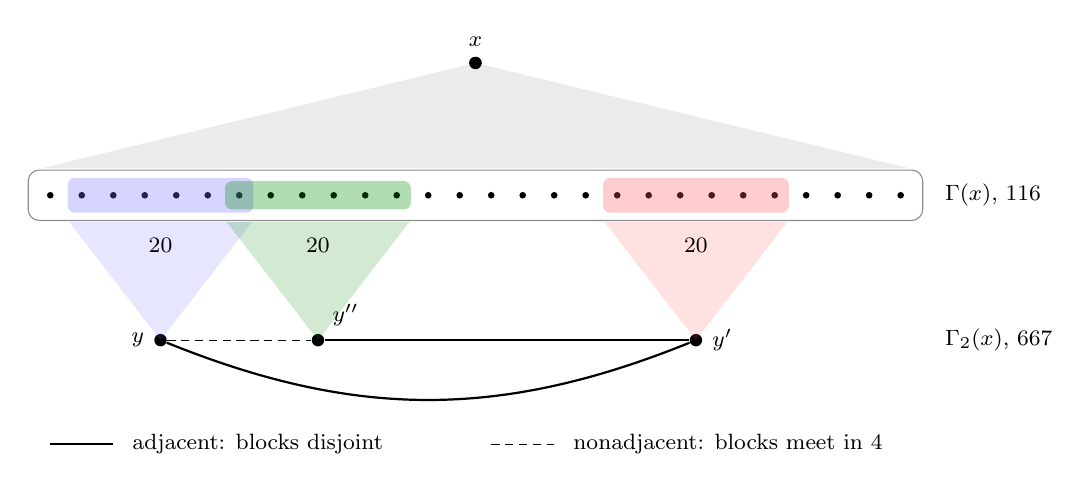
\begin{tikzpicture}[x=0.4cm,y=0.4cm,
  dot/.style={circle,fill=black,inner sep=0pt,minimum size=2.4pt},
  vtx/.style={circle,fill=black,inner sep=0pt,minimum size=4.5pt},
  lab/.style={font=\footnotesize},
  blk/.style={rounded corners=2.5pt,inner sep=0pt}]
  % the 116 neighbors of x, drawn as 28 dots
  \draw[black!45,rounded corners=4pt] (-0.7,-0.8) rectangle (27.7,0.8);
  \foreach \i in {0,...,27} \node[dot] (n\i) at (\i,0) {};
  % three blocks B_y, B_{y''}, B_{y'}
  \fill[blue!55,opacity=.30,blk] (0.55,-0.55) rectangle (6.45,0.55);
  \fill[green!55!black,opacity=.30,blk] (5.55,-0.45) rectangle (11.45,0.45);
  \fill[red!65,opacity=.30,blk] (17.55,-0.55) rectangle (23.45,0.55);
  % x above, joined to every neighbor
  \node[vtx,label={[lab]above:$x$}] (x) at (13.5,4.2) {};
  \fill[black!8] (x.center) -- (-0.3,0.85) -- (27.3,0.85) -- cycle;
  \node[vtx] at (x) {};
  % three vertices at distance 2, each joined to its block of 20
  \node[vtx,label={[lab]left:$y$}] (y) at (3.5,-4.6) {};
  \node[vtx,label={[lab]above right:$y''$}] (yy) at (8.5,-4.6) {};
  \node[vtx,label={[lab]right:$y'$}] (y1) at (20.5,-4.6) {};
  \fill[blue!55,opacity=.18] (y.center) -- (0.6,-0.85) -- (6.4,-0.85) -- cycle;
  \fill[green!55!black,opacity=.18] (yy.center) -- (5.6,-0.85) -- (11.4,-0.85) -- cycle;
  \fill[red!65,opacity=.18] (y1.center) -- (17.6,-0.85) -- (23.4,-0.85) -- cycle;
  \draw[thick] (yy) -- (y1);
  \draw[thick] (y) to[bend right=22] (y1);
  \draw[densely dashed] (y) -- (yy);
  % labels
  \node[lab,anchor=west] at (28.1,0) {$\Gamma(x)$, $116$};
  \node[lab,anchor=west] at (28.1,-4.6) {$\Gamma_2(x)$, $667$};
  \foreach \c in {3.5,8.5,20.5} \node[lab] at (\c,-1.6) {$20$};
  % key
  \draw[thick] (0,-7.9) -- (2,-7.9);
  \node[lab,anchor=west] at (2.3,-7.9) {adjacent: blocks disjoint};
  \draw[densely dashed] (14,-7.9) -- (16,-7.9);
  \node[lab,anchor=west] at (16.3,-7.9) {nonadjacent: blocks meet in $4$};
\end{tikzpicture}
\caption{A putative $\Kre(4)=\mathrm{srg}(784,116,0,20)$ seen from a
vertex $x$, with three of the $667$ vertices at distance two. The
neighborhood $\Gamma(x)$ has no edges; each dot stands for about four of
its points. Each $y$ at distance two has $20$ neighbors $B_y\subset\Gamma(x)$,
and the distance-two graph $\Gamma_2(x)$ is an $\mathrm{srg}(667,96,0,16)$.
The blocks $B_y$ form a $3$-$(116,20,3)$ design (\S\ref{sec:sub}).}\label{fig:kre4}
\end{figure}

\paragraph{Relation to earlier work, and scope.}
Bannai, Munemasa and Venkov \cite{BMV} and Nebe and Venkov \cite{NV} excluded
tight spherical designs using the integral lattices spanned by the designs
together with their design strength \cite{Venkov}; characteristic vectors and
van der Blij's congruence already appear there. Kova\v l \cite{Koval}
adapted this to strongly regular graphs through discriminant forms; at
$392$, $784$ and $1080$ his census admits $4$, $4$ and $16$ discriminant forms,
respectively, in each of the two representations (on the $r$- and on the
$s$-eigenspace side). For distance-regular graphs, Krein equality has been used
combinatorially, through triple intersection numbers \cite{CJ,GVW}. Euclidean representations have also been combined with algebraic
identities to exclude individual strongly regular graphs, for example
$(76,30,8,14)$ \cite{BPR}. The new ingredient here is that we use the
\emph{odd} third moment arithmetically. For odd $x$ one has
$x^3-x\equiv x^2-1\pmod{16}$; applied to the inner products of a characteristic
vector with the vertex vectors, this lifts the frame congruence for $Fw^2$
from modulus $8$ to modulus $16$. When $v_2(F)\le2$ the extra factor of $2$
forces every maximal integral lattice containing the vertex vectors to be
unimodular at $2$, and van der Blij's congruence for
characteristic norms \cite{vdB} then gives the contradiction. The methods are
complementary: none of the $135$ Smith parameter sets with $r\le135$ that
would give tight spherical $4$-designs, where \cite{BMV} applies, is excluded
here.

For each $r$ there are finitely many Smith parameter sets
(Lemma~\ref{lem:param}); with $r\le135$ there are $2320$.
Theorem~\ref{thm:main} and a variant at one vertex (Theorem~\ref{thm:vertex})
exclude $77$ of them (for $\Kre(t)$ we compute $\Delta$ from the neighbor
basis), of which $71$ pass the standard feasibility checks
(\S\ref{sec:baseline}). For $43$ of these $71$, a second-moment test
(Proposition~\ref{prop:second}) gives no exclusion, whether applied to the
graph or to its subconstituents. These $43$ include $392$, $784$, $1080$ and every $\Kre(t)$ with $t\le135$,
$t\equiv4\pmod 8$ (Figure~\ref{fig:reach}).

Sections~\ref{sec:lattices}--\ref{sec:srg} prove Theorem~\ref{thm:main},
\S\ref{sec:apps} gives its applications and the second subconstituent, \S\ref{sec:vertex} the vertex
variant, \S\ref{sec:second} explicit families from the second moment alone, and
\S\ref{sec:drg} distance-regular graphs. The nonexistence theorems have
arithmetic proofs. Section~\ref{sec:checks} describes the finite censuses and
their reproducibility checks.

%======================================================================
\section{Lattices at the prime 2}\label{sec:lattices}

Let $\Zt$ be the ring of rational numbers with odd denominator; $v_2$ and
$\odd$ are as in \S\ref{sec:intro}. Residues of elements of $\Zt$ modulo $2^j$ are taken in
$\Zt/2^j\Zt\cong\Z/2^j$.

Let $U$ be a positive definite rational quadratic space of dimension $m$, with
form $\ip{\cdot}{\cdot}$, and write $x^2=\ip xx$. A \emph{lattice} is a
finitely generated $\Zt$-submodule $N\subset U$ that spans $U$. (In
Lemma~\ref{lem:det} we also use $\Z$-lattices, and say so.) It is free of rank
$m$, and its determinant $\det N$, the determinant of the Gram matrix of a
basis, is well defined up to squares of units and lies in the square class of
$\det U$. Odd squares are $\equiv1\pmod 8$, so
\[
 \Delta(U):=\odd(\det U)\bmod 4\ \in\{1,3\}
\]
is well defined; it can be computed from the Gram matrix of any basis of $U$.
\begin{itemize}
\item $N$ is \emph{integral} if $\ip xy\in\Zt$ for all $x,y\in N$, and
\emph{even} if moreover $x^2\in2\Zt$ for all $x\in N$.
\item The \emph{dual} of $N$ is $N^\#=\{x\in U:\ip xN\subseteq\Zt\}$; $N$ is
\emph{unimodular} if $N^\#=N$, that is, if $\det N$ is a unit.
\item A vector $w\in N$ is \emph{characteristic} if $\ip wx\equiv x^2\pmod 2$
for all $x\in N$. For example, in $\Z^m$ the vector $(1,\dots,1)$ is
characteristic, with norm $m$; this matches Lemma~\ref{lem:charnorm} with
$\Delta=1$.
\end{itemize}

We use three standard facts.
\begin{enumerate}[label=(L\arabic*)]
\item \emph{Maximal lattices exist.} If $N$ is integral, every integral lattice
containing $N$ lies in $N^\#$, and $N^\#/N$ is finite. Hence $N$ is contained in
a maximal integral lattice.
\item \emph{Characteristic vectors exist.} Let $N$ be integral. The map
$x\mapsto x^2\bmod2$ is linear on $N/2N$ and vanishes on the radical of the
reduced form, so it has the form $x\mapsto\ip wx\bmod 2$ for some $w\in N$.
\item \emph{Jordan splitting} \cite[\S\S91--93]{OMeara},
\cite[Ch.~8]{Cassels}. (These results are proved over the $2$-adic integers;
the splittings we need, splitting off a sublattice whose Gram determinant is a
unit, work verbatim over $\Zt$.)
\begin{itemize}
\item An integral lattice $N$ with $2N^\#\subseteq N$ is an orthogonal sum
$N=N_0\perp N_1$ with $N_0$ unimodular and $N_1^\#=\tfrac12N_1$.
\item A unimodular lattice is an orthogonal sum of lines $\langle\alpha\rangle$
with $\alpha$ odd and of planes with Gram matrix
$\left(\begin{smallmatrix}2\alpha&\beta\\ \beta&2\gamma\end{smallmatrix}\right)$,
$\beta$ odd. Each such plane has determinant $\equiv-1\pmod 4$.
\item A unimodular lattice is even if and only if no lines occur. Then its rank
is even, say $2p$, and its determinant is $\equiv(-1)^p\pmod4$.
\end{itemize}
\end{enumerate}

\begin{lemma}[characteristic norm]\label{lem:charnorm}
Let $N$ be a unimodular lattice in $U$ and $w\in N$ characteristic. Then
$w^2\equiv m+1-\Delta(U)\pmod 4$.
\end{lemma}

This is the reduction modulo $4$ of van der Blij's theorem that $w^2$ is
congruent modulo $8$ to the oddity \cite{vdB}; see \cite[Ch.~II]{MH},
\cite[Ch.~15]{CS}.

\begin{proof}
By (L3), write $N=\langle y_1\rangle\perp\dots\perp\langle y_j\rangle\perp N_0$
with $\alpha_i=y_i^2$ odd and $N_0$ even unimodular of rank $2p$, so $m=j+2p$.
Write $w=\sum c_iy_i+w_0$ with $w_0\in N_0$. Each $c_i$ is odd, since
$c_i\alpha_i=\ip w{y_i}\equiv\alpha_i$. And $w_0$ is characteristic for the
even lattice $N_0$, so $w_0\in2N_0^\#=2N_0$ and $w_0^2\in8\Zt$. Hence
$w^2\equiv\sum_ic_i^2\alpha_i\equiv\sum_i\alpha_i\pmod 8$.

The determinant satisfies $\Delta\equiv(-1)^p\prod_i\alpha_i\pmod 4$. For odd
$x,y$ we have $1-xy\equiv(1-x)+(1-y)\pmod 4$, so
$1-\Delta\equiv2p+\sum_i(1-\alpha_i)$. Therefore
$\sum_i\alpha_i\equiv m-1+\Delta\equiv m+1-\Delta\pmod 4$, using
$2\Delta\equiv2$.
\end{proof}

%======================================================================
\section{Integral tight frames}\label{sec:frames}

Let $v_1,\dots,v_n$ span $U$ and have integral Gram matrix
$G=(\ip{v_i}{v_j})$. Suppose they form a \emph{tight frame} with constant
$F>0$:
\begin{equation}\label{eq:frame}
 \sum_i\ip x{v_i}\ip y{v_i}=F\ip xy\qquad(x,y\in U),
\end{equation}
or equivalently $G^2=FG$. Then $m=\operatorname{tr}G/F$. The \emph{first
moment} vanishes if $\sum_iv_i=0$, and the \emph{third moment} vanishes if
$\sum_i\ip x{v_i}^3=0$ for all $x\in U$, equivalently
$\sum_{i,j}G_{ij}^3=0$ (indeed $\|\sum_iv_i\otimes v_i\otimes v_i\|^2=
\sum_{i,j}G_{ij}^3$, and a symmetric tensor vanishes if and only if its cubic
form does).

\begin{theorem}\label{thm:frame}
Let $N\supseteq\sum_i\Zt v_i$ be a maximal integral lattice and $w\in N$ a
characteristic vector. Define $(T,M)$ as follows.
\begin{enumerate}[label=\textup{(\alph*)}]
\item If every $v_i^2$ is odd, $(T,M)=(n,8)$.
\item If, as in (a), every $v_i^2$ is odd, and moreover the first and third
moments vanish, $(T,M)=(n,16)$.
\item If every $v_i^2$ is even and the first moment vanishes, $(T,M)=(0,8)$.
\end{enumerate}
Then $Fw^2\equiv T\pmod M$. If $v_2(F)\le v_2(M)-2$, then $v_2(T)\ge v_2(F)$,
$N$ is unimodular, $v_2(\det U)$ is even, and
\[
 T/F\equiv m+1-\Delta(U)\pmod 4 .
\]
\end{theorem}

\begin{proof}
Let $z\in N^\#$ and put $x_i=\ip{w+2z}{v_i}\in\Zt$. Since $v_i\in N$, we have
$\ip w{v_i}\equiv v_i^2$, so $x_i\equiv v_i^2\pmod 2$. By \eqref{eq:frame},
$\sum_ix_i^2=F(w+2z)^2$. We evaluate this sum in each case.
\begin{itemize}
\item[(a)] Each $x_i$ is odd, so $x_i^2\equiv1\pmod 8$.
\item[(b)] For odd $x$, $(x^3-x)-(x^2-1)=(x-1)(x^2-1)\in16\Zt$. The vanishing
moments give $\sum x_i=\sum x_i^3=0$. Hence
$\sum_i x_i^2\equiv n+\sum_i(x_i^3-x_i)=n\pmod{16}$.
\item[(c)] Write $x_i=2y_i$. Then $\sum y_i=0$, and $y^2\equiv y\pmod 2$, so
$\sum x_i^2=4\sum y_i^2\equiv4\sum y_i=0\pmod 8$.
\end{itemize}
Thus $F(w+2z)^2\equiv T\pmod M$ for every $z\in N^\#$, and $z=0$ gives the
first claim. Subtracting the two congruences gives
$4F\bigl(\ip wz+z^2\bigr)\in M\Zt$.

Suppose $v_2(F)\le v_2(M)-2$. Then $\ip wz+z^2\in\Zt$. Also $\ip wz\in\Zt$, since
$w\in N$ and $z\in N^\#$; so $z^2\in\Zt$. Then $N+\Zt z$ is integral, and
maximality gives $z\in N$. Hence $N^\#=N$, $\det N$ is a unit, and
$v_2(\det U)$ is even.

Finally, write $\delta=v_2(F)$. From $Fw^2\equiv T\pmod M$ with $w^2\in\Zt$ and
$\delta<v_2(M)$ we get $v_2(T)\ge\delta$. Writing $F=2^\delta F'$ and
$T=2^\delta T'$, we have
$F'w^2\equiv T'\pmod{2^{v_2(M)-\delta}}$ with $v_2(M)-\delta\ge2$, so
$w^2\equiv T/F\pmod 4$. Now apply Lemma~\ref{lem:charnorm}.
\end{proof}

To use Theorem~\ref{thm:frame} one needs $\Delta(U)$. For frames with constant
diagonal it is largely determined by arithmetic.

\begin{lemma}[determinant]\label{lem:det}
Suppose all diagonal entries of $G$ are equal to $\eta$. Let $c>0$ be the
gcd of all differences $G_{ij}-\eta$, and assume $\gcd(\eta,c)=1$. Let $\nu$
be the numerator of $F/c$, or of $F/c^2$ if the third moment vanishes. Then
$c^{m+1}\det U$ is a positive divisor of $\nu$ times a rational square.
In particular, if every odd prime divisor of $\nu$ is $\equiv1\pmod 4$, then
$\Delta(U)\equiv\odd(c)^{m+1}\pmod 4$. If, in addition, $\nu$ is odd, then
$v_2(\det U)\equiv(m+1)v_2(c)\pmod 2$.
\end{lemma}

\begin{proof}
Let $B=c^{-1}\ip{\cdot}{\cdot}$, let $\Lambda=\sum\Z v_i$ (a $\Z$-lattice of full
rank), and let $\Lambda^*=\{x:B(x,\Lambda)\subseteq\Z\}$ be its dual with respect to $B$.
Every value $B(v_i,v_j)$ is $\equiv\eta/c\pmod\Z$, and \eqref{eq:frame} becomes
$\sum_iB(x,v_i)B(y,v_i)=(F/c)B(x,y)$. Hence $(F/c)B(x,y)\in\Z$ for all
$x,y\in \Lambda^*$.

Suppose the third moment vanishes. Contracting $\sum_iv_i^{\otimes3}=0$ with
$v_j\otimes x\otimes y$ gives
\[
 \sum_iB(v_i,v_j)\,B(x,v_i)\,B(y,v_i)=0 .
\]
Since $B(v_i,v_j)-\eta/c\in\Z$, the left side is
$(\eta/c)(F/c)B(x,y)$ plus an integer, so $(\eta/c)(F/c)B(x,y)\in\Z$. Together
with $(F/c)B(x,y)\in\Z$ and $\gcd(\eta,c)=1$, this gives
$(F/c^2)B(x,y)\in\Z$. So in both cases $\nu B(x,y)\in\Z$ for $x,y\in \Lambda^*$.

Now fix a prime $\ell\nmid\nu$ and localize at $\ell$. (Localization commutes
with taking duals of full-rank lattices.)
\begin{itemize}
\item $\Lambda^*_\ell$ is $B$-integral, so $\Lambda^*_\ell\subseteq \Lambda_\ell$.
\item Consider the map $\Lambda_\ell\to\Q/\Z_{(\ell)}$ sending $\sum \beta_iv_i$ to
$B(\sum \beta_iv_i,v_j)$. Modulo $\Z_{(\ell)}$ this equals $(\eta/c)\sum \beta_i$, so it
does not depend on $j$. Its kernel is therefore $\Lambda_\ell\cap \Lambda^*_\ell=\Lambda^*_\ell$,
and its image has order $\ell^{v_\ell(c)}$.
\item Hence $[\Lambda_\ell:\Lambda^*_\ell]=\ell^{v_\ell(c)}$. Since
$\det_B\Lambda^*=(\det_B\Lambda)^{-1}$ and $\det_B\Lambda^*=[\Lambda:\Lambda^*]^2\det_B\Lambda$, we get
$v_\ell(\det_B\Lambda)=-v_\ell(c)$.
\end{itemize}
Modulo squares $\det U=c^m\det_B\Lambda$, so $v_\ell(\det U)\equiv(m+1)v_\ell(c)$ for
every prime $\ell\nmid\nu$, and $\det U>0$. This is the claim.
\end{proof}

%======================================================================
\section{Strongly regular graphs}\label{sec:srg}

Let $\Gamma$ be as in \S\ref{sec:intro}, with $e=r-s$ and $u=(k-r)/n=a/b$, and
put $H=rI-A+uJ$. Then $H$ vanishes on the all-ones vector and on the
$r$-eigenspace, and acts as $e$ on the $s$-eigenspace. So $H=e\cdot E_s$:
$H^2=eH$, $\operatorname{rank}H=g$, and $H$ is positive semidefinite.

Let $U$ be the column space of $H$ with the form $\ip{Hx}{Hy}=x^\top Hy$, and
let $p_i$ be the $i$-th column of $H$. Then $\ip{p_i}{p_j}=H_{ij}$, $\sum_ip_i=0$, and the $p_i$ form
a tight frame with constant $e$. Comparing diagonals in $H^2=eH$ gives
\begin{equation}\label{eq:diag}
 nu(1-u)=e(r+u)-r(r+1).
\end{equation}
The matrix $bH$ is the Gram matrix of the $p_i$ in the space $U_b$ obtained
from $U$ by multiplying the form by $b$. Its entries are integers: $br+a$ on
the diagonal, $a$ for nonadjacent pairs and $a-b$ for adjacent pairs. Its frame
constant is $F=be$. Any nonsingular $g\times g$ principal submatrix of $bH$ is
the Gram matrix of a basis of $U_b$, so the $\Delta$ of
Theorem~\ref{thm:main} is $\Delta(U_b)$. Finally,
$\operatorname{tr}(bH)=n(br+a)$ and $\operatorname{tr}(bH)=F\operatorname{rank}H=Fg$, so
\begin{equation}\label{eq:trace}
 g=(br+a)\,\frac nF .
\end{equation}

\subsection{Krein equality}

\begin{proposition}\label{prop:krein}
We have
\[
 \frac{e^3g}n\,q^s_{ss}=\sum_{i,j}H_{ij}^3=n(r+u)\bigl[r(r+1)-(1-2u)e\bigr].
\]
Hence $q^s_{ss}=0$ if and only if $e(1-2u)=r(r+1)$. In that case the third
moment of the $p_i$ vanishes.
\end{proposition}

\begin{proof}
We have
$\sum_{ij}(E_s)_{ij}^3=\operatorname{tr}((E_s\circ E_s)E_s)=q^s_{ss}\operatorname{tr}(E_s)/n$
by the definition of $q^s_{ss}$, and $H=eE_s$. For the second equality put
$x=r+u$, the diagonal entry of $H$. The off-diagonal entries $y\in\{u,u-1\}$
satisfy $y^2=(2u-1)y-u(u-1)$, hence $y^3=(2u-1)y^2-u(u-1)y$. In each row the
off-diagonal entries sum to $-x$ (as $H\mathbf 1=0$) and their squares sum to
$ex-x^2$ (as $H^2=eH$). So each row contributes
\[
 x^3+(2u-1)(ex-x^2)+u(u-1)x=x\bigl[(x-u)(x-u+1)-(1-2u)e\bigr],
\]
and $x-u=r$. Finally $r+u=eg/n>0$.
\end{proof}

\begin{lemma}[Smith parameter sets]\label{lem:param}
Fix $r\ge1$ and put $h=e-r(r+1)$; by Proposition~\ref{prop:krein},
$h=2eu>0$.
\begin{enumerate}[label=\textup{(\roman*)}]
\item The Smith parameter sets with positive eigenvalue $r$ are given by
\[
 u=\frac h{2e},\qquad
 n=\frac{2e^2\bigl(e(2r+1)-3r(r+1)\bigr)}{h\,(2r(r+1)+h)},\qquad k=r+nu,
\]
with $\mu=k+rs$ and $\lambda=\mu+r+s$.
\item Integrality of $n$ forces $h\mid4r^3(r+1)^3(r-1)$ for $r\ge2$, and
$(e+2)\mid24$ for $r=1$. So there are finitely many sets for each $r$.
\item For fixed $u=a/b$ and $r=t$ they are
\[
 e=\frac{bt(t+1)}{b-2a},\qquad
 n=\frac{b^2t(t+1)(bt+3a-b)}{(b-2a)a(b-a)},\qquad
 g=\frac{(bt+3a-b)(bt+a)}{a(b-a)}.
\]
\item In all cases $n>4r(r^2-1)$.
\end{enumerate}
\end{lemma}

\begin{proof}
(i) and (iii) follow by solving $e(1-2u)=r(r+1)$ together with \eqref{eq:diag}
and $g=n(r+u)/e$. For (ii), reduce the numerator of $n$ modulo $h$: since
$e\equiv r(r+1)$, it is $\equiv4r^3(r+1)^3(r-1)$. For $r=1$ the formula reduces
to $n=6e^2/(e+2)$. For (iv), write $e=xr(r+1)$ with $x>1$. Then
$n=2r(r+1)x^2\bigl(x(2r+1)-3\bigr)/(x^2-1)>2r(r+1)(2r-2)$.
\end{proof}

\begin{proof}[Proof of Theorem~\ref{thm:main}]
The vectors $p_i$ in $U_b$ have norm $br+a$, and by
Proposition~\ref{prop:krein} their first and third moments vanish. If $br+a$
is odd, Theorem~\ref{thm:frame}(b) applies, with $(T,M)=(n,16)$ and
$v_2(F)\le2$; it gives $n/F\equiv g+1-\Delta$, and substituting
\eqref{eq:trace} gives (a). If $br+a$ is even, Theorem~\ref{thm:frame}(c)
applies, with $(T,M)=(0,8)$ and $v_2(F)\le1$; it gives $0\equiv g+1-\Delta$,
which is (b). For (c), apply Lemma~\ref{lem:det} to $bH$. The differences of entries are
$-br$ and $-b(r+1)$, so $c=b$, and $\gcd(br+a,b)=1$. The third moment vanishes,
so $\nu$ is the numerator of $F/c^2=e/b$, that is, $\nu=L$.
\end{proof}

The next identity is the contraction of the vanishing third moment with a
single vertex. It is used in \S\ref{sec:vertex}.

\begin{lemma}[neighborhood identity]\label{lem:nbhd}
If $q^s_{ss}=0$ and $d=eu$, then for every vertex $x$ and all $y,z\in U$,
\[
 \sum_{i\sim x}\ip y{p_i}\ip z{p_i}=d\,\ip yz+r\,\ip y{p_x}\ip z{p_x}.
\]
\end{lemma}

\begin{proof}
The third moment vanishes (Proposition~\ref{prop:krein}), so by polarization
$\sum_i\ip{p_i}{p_x}\ip y{p_i}\ip z{p_i}=0$. Substituting
$\ip{p_i}{p_x}=r\delta_{ix}-A_{ix}+u$ and using \eqref{eq:frame} gives
\[
 0=r\ip y{p_x}\ip z{p_x}-\sum_{i\sim x}\ip y{p_i}\ip z{p_i}+ue\ip yz .
 \qedhere
\]
\end{proof}

\subsection{The second-moment test}\label{sec:baseline}
Without Krein equality, Theorem~\ref{thm:frame}(a),(c) and Lemma~\ref{lem:det}
still apply to $bH$, now with $\nu=e$, the numerator of $F/b$.

\begin{proposition}\label{prop:second}
Let $\Gamma$ be a primitive strongly regular graph with integral eigenvalues.
Suppose $v_2(F)\le1$ and every odd prime divisor of $e$ is $\equiv1\pmod 4$.
Then
\[
 \odd(b)^{g+1}\equiv\begin{cases}1+(br+a-1)\,n/F&(br+a\ \text{odd}),\\
 1+g&(br+a\ \text{even})\end{cases}\pmod 4 .
\]
\end{proposition}

\begin{proof}
Theorem~\ref{thm:frame}(a),(c) give $n/F\equiv g+1-\Delta$ and
$0\equiv g+1-\Delta$, Lemma~\ref{lem:det} with $\nu=e$ gives
$\Delta\equiv\odd(b)^{g+1}$, and we substitute \eqref{eq:trace}.
\end{proof}

This is a special case of the discriminant-form method \cite{BMV,Koval}. On
Brouwer's table it excludes $154$ rows ($77$ complementary pairs), all already
marked nonexistent. Among them are rows whose nonexistence was first proved
by much longer arguments; Table~\ref{tab:known} gives the data that make each
of them a two-line check. In every row the odd prime divisors of $e$ are
$\equiv1\pmod 4$ and $v_2(F)\le1$.
\begin{table}[ht]\small\centering
\caption{Known nonexistence results reproved by
Proposition~\ref{prop:second}. The last two columns must agree modulo $4$;
the requirement is $1+(br+a-1)n/F$ if $br+a$ is odd and $1+g$ if it is
even.}\label{tab:known}
\setlength{\tabcolsep}{5pt}
\begin{tabular}{lcccccccc}\toprule
parameters&$e$&$u$&$br+a$&$F$&$n/F$&$g$&requirement&$\odd(b)^{g+1}$\\\midrule
$(75,32,10,16)$ \cite{AM}&$10$&$2/5$&$12$&$50$&$3/2$&$18$&$1+18\equiv3$&$5^{19}\equiv1$\\
$(76,35,18,14)$ \cite{AM}&$10$&$7/19$&$140$&$190$&$2/5$&$56$&$1+56\equiv1$&$19^{57}\equiv3$\\
$(76,30,8,14)$ \cite{BPR}&$10$&$7/19$&$45$&$190$&$2/5$&$18$&$1+44\cdot\frac25\equiv1$&$19^{19}\equiv3$\\
$(289,54,1,12)$ \cite{BR}&$17$&$3/17$&$54$&$289$&$1$&$54$&$1+54\equiv3$&$17^{55}\equiv1$\\
\bottomrule
\end{tabular}
\end{table} For a Smith graph the subconstituents are strongly regular
with forced parameters \cite{CGS}, with eigenvalues $r,\,r-d$ and
$r,\,r-(e-d)$, so Proposition~\ref{prop:second} applies to them as well.

\paragraph{Conventions.} We say that a parameter set has a \emph{Proposition
\ref{prop:second} exclusion} if Proposition~\ref{prop:second} fails for the
graph or its complement or, for a Smith set, for either nontrivial
subconstituent or its complement. This is the baseline against which we mark our
exclusions; it does not show that every second-moment argument fails. A Smith
parameter set \emph{passes the feasibility checks} if it satisfies
integrality, the Krein conditions and the absolute bound
$n\le\frac12f(f+3)$, $n\le\frac12g(g+3)$, its forced local
eigenvalue gaps $d$ and $e-d$ are integers, and each nontrivial subconstituent
satisfies the same conditions or is a disjoint union of equal cliques or the
complement of one.

\begin{remark}\label{rem:sharp}
The hypothesis on $L$ in Theorem~\ref{thm:main}(c) cannot be dropped. The
second subconstituent of the McLaughlin graph, $\mathrm{srg}(162,56,10,24)$, is
a Smith graph with $r=2$, $s=-16$, $u=1/3$, $br+a=7$, $F=54$, $n/F=3$, $g=21$
and $L=6$. Part (a) gives $\Delta\equiv1+6\cdot3\equiv3$, whereas
$\odd(b)^{g+1}=3^{22}\equiv1$; since the graph exists, $\Delta=3$, and the
formula in (c) fails because $3\mid L$.
\end{remark}

%======================================================================
\section{Applications}\label{sec:apps}

\subsection{The three table rows with Krein equality}
In each row below Krein equality holds, $br+a$ is odd and $v_2(F)=2$, so
Theorem~\ref{thm:main}(a) requires $\Delta\equiv1+(br+a-1)n/F$. No $L$ has a
prime divisor $\equiv3\pmod4$, so by (c) $\Delta\equiv b^{g+1}$.
\begin{center}\setlength{\tabcolsep}{4pt}
\begin{tabular}{rrrrrrrrrrrcc}\toprule
$n$&$k$&$\lambda$&$\mu$&$r$&$s$&$u$&$br+a$&$F$&$n/F$&$g$&$1+(br+a-1)\frac nF$&$b^{g+1}$\\
\midrule
392&115&18&40&3&$-25$&$2/7$&23&196&2&46&$1+44\equiv1$&$7^{47}\equiv3$\\
784&116&0&20&4&$-24$&$1/7$&29&196&4&116&$1+112\equiv1$&$7^{117}\equiv3$\\
1080&364&88&140&4&$-56$&$1/3$&13&180&6&78&$1+72\equiv1$&$3^{79}\equiv3$\\
\bottomrule
\end{tabular}
\end{center}
This proves the case $t=4$ of Theorem~\ref{thm:headline}(a) and (c); a graph
exists if and only if its complement does. Of their subconstituents,
$(667,96,0,16)$ is excluded in \S\ref{sec:sub}, and $(115,18,1,3)$,
$(276,75,10,24)$, $(364,88,12,24)$ and $(715,224,48,80)$ remain open
\cite{Tab}.

\subsection{Triangle-free Krein graphs}

\begin{proof}[Proof of Theorem~\ref{thm:headline}(a)]
For $\Kre(t)$ we have $e=t(t+3)$, $u=1/(t+3)$, $br+a=e+1$ (odd),
$F=t(t+3)^2$, $n/F=t$ and $g=k$. If $t\equiv4\pmod 8$, then $v_2(F)=2$, and
Theorem~\ref{thm:main}(a) requires $\Delta\equiv1+et\equiv1\pmod 4$.
On the other hand, since $\lambda=0$ the $k$ neighbors of a vertex have Gram
matrix $eI+J$ in $bH$. This matrix is nonsingular of size $k=g$, so the
neighbors form a rational basis of $U_b$, and
\[
 \det U_b\equiv e^{k-1}(e+k)=e^{k-1}\,t(t+2)^2 .
\]
Since $t$ and hence $k=t(e+1)$ are even, this is $(t+3)$ times a square, so
$\Delta\equiv t+3\equiv3$, a contradiction.
\end{proof}

The same computation decides every $t$. For even $t$ we have
$\Delta\equiv t+3$; Theorem~\ref{thm:main}(a) applies when $8\nmid t$ and
requires $\Delta\equiv1+et\equiv1$, which fails exactly for $t\equiv4\pmod 8$.
For odd $t$ the neighbor basis gives $\Delta\equiv t\equiv1+et$, so
Theorem~\ref{thm:main} (whose part (a) applies when $t\equiv3\pmod 4$) never excludes
$\Kre(t)$. Neither does Theorem~\ref{thm:vertex} below ($b=t+3$ is even):
there $\det W$ lies in the square class of the odd number $k=g$, and
$k\equiv(-1)^{(k-1)/2}\pmod 4$ holds for every odd $k$. So $\Kre(3)$, which
does not exist \cite{GM,KO}, is not excluded by our congruences.

\begin{proof}[Proof of Theorem~\ref{thm:headline}(b)]
Let $\mathcal D$ be a $3$-$(v,K,t-1)$ design with $v=t(t^2+3t+1)$ and
$K=t(t+1)$. Counting gives pair multiplicity $K-1$, replication number $v-1$,
and $v(v-1)/K$ blocks. Deriving at a point gives a symmetric
$2$-$(v-1,K-1,t-1)$ design, so any two blocks meet in $0$ or $t$ points.

Two equal blocks through a point would give a repeated block of the
derived symmetric design, which is impossible, so the blocks are distinct.
Let $N$ be the point--block incidence matrix, $D_0$ the disjointness matrix
of the blocks and $X=N^\top N$; we write $J$ for any all-ones matrix. Then
\[
 NN^\top=(v-K)I+(K-1)J,\quad NJ=(v-1)J,\quad JN=KJ,\quad X=t(tI+J-D_0),
\]
the last because $K-t=t^2$. Hence $D_0=tI+J-X/t$ and
$X^2=N^\top(NN^\top)N=(v-K)X+(K-1)K^2J$. Substituting, and using
$v-K=t^2(t+2)$ and $K(K-1)=t(t+1)(t^2+t-1)$, one finds that the coefficients
of $J$ cancel and
\[
 ND_0=K(J-N),\qquad D_0^2+X=t^2I+(t+1)X=(v-K)I-KD_0+KJ .
\]

Now form a graph whose vertices are a root, the points and the blocks. Join
the root to every point, each point to the blocks containing it, and each
block to the blocks disjoint from it. By the identities above, its adjacency
matrix satisfies $A^2=(v-K)I-KA+KJ$. So it is a strongly regular graph with
parameters $(t^2(t+3)^2,v,0,K)$, that is, $\Kre(t)$, which does not exist by
part (a).
\end{proof}

For $t=2$ this is the classical construction of the Higman--Sims graph from the
Witt design $3$-$(22,6,1)$. Conversely, the neighbors of a vertex of $\Kre(t)$,
with the sets $\Gamma(x)\cap\Gamma(y)$ as blocks, form such a design, since
triple intersection numbers are constant at Krein equality \cite{CGS}; see
also \cite{CMN}. With $\lambda=t-1$ the derived designs are
$2$-$\bigl((\lambda+2)(\lambda^2+4\lambda+2),\lambda^2+3\lambda+1,\lambda\bigr)$
designs, the second of Cameron's families \cite{Cameron}.

\subsection{The second subconstituent}\label{sec:sub}
Fix $t\ge1$ and put $v=t(t^2+3t+1)$ and $K=t(t+1)$, as in
Theorem~\ref{thm:headline}(b). In $\Kre(t)$ the non-neighbors of a vertex $x$
induce a strongly regular graph with parameters
\begin{equation}\label{eq:sub}
 (n,k,\lambda,\mu)=\bigl((t^2+2t-1)(t^2+3t+1),\ t^2(t+2),\ 0,\ t^2\bigr)
\end{equation}
\cite[\S8.5]{BvM} (see also \cite{Biggs3}), and two such vertices $y,y'$ are
adjacent if and only if the blocks $\Gamma(x)\cap\Gamma(y)$ and
$\Gamma(x)\cap\Gamma(y')$ of the design in Theorem~\ref{thm:headline}(b) are
disjoint (Figure~\ref{fig:kre4}). We show that the graph alone determines the
design. For $t=2$, where \eqref{eq:sub} is $(77,16,0,4)$, this is classical
\cite{Br77}. For $t=1$, where \eqref{eq:sub} is the Petersen graph, the
``design'' degenerates: the proof below reconstructs ten distinct $2$-subsets
of a $5$-set, that is, all of them, and the Petersen graph is their
disjointness graph.

\begin{theorem}\label{thm:sub}
Let $t\ge2$. Every strongly regular graph with parameters \eqref{eq:sub} is
the disjointness graph of the blocks of a $3$-$(v,K,t-1)$ design.
\end{theorem}

\begin{corollary}\label{cor:equiv}
For every $t\ge2$ the following are equivalent: \textup{(i)} a strongly
regular graph with parameters \eqref{eq:sub} exists; \textup{(ii)} a
$3$-$(v,K,t-1)$ design exists; \textup{(iii)} $\Kre(t)$ exists. In
particular there is no $\mathrm{srg}(266,45,0,9)$, and none with parameters
\eqref{eq:sub} for $t\equiv4\pmod 8$.
\end{corollary}

\begin{proof}
(i)$\Rightarrow$(ii) is Theorem~\ref{thm:sub}; (ii)$\Rightarrow$(iii) is the
construction in the proof of Theorem~\ref{thm:headline}(b), which does not
use $t\equiv4\pmod 8$; and (iii)$\Rightarrow$(i) holds because the second
subconstituent of $\Kre(t)$ has parameters \eqref{eq:sub}. At $t=3$ a graph
$\mathrm{srg}(266,45,0,9)$ would give a $3$-$(57,12,2)$ design and hence
$\Kre(3)$, contradicting \cite{GM,KO}; for $t\equiv4\pmod 8$ use
Theorem~\ref{thm:headline}(a).
\end{proof}

This proves Theorem~\ref{thm:headline}(d); the complement $(667,570,489,475)$
of the case $t=4$ is excluded with it. Brouwer's table credits the
nonexistence of $\mathrm{srg}(266,45,0,9)$ to Akiyama \cite{Akiyama}, whose
formalized proof is a long lattice argument. The proof above is short given
the nonexistence of a $3$-$(57,12,2)$ design, that is, of $\Kre(3)$, which was
proved by Gavrilyuk and Makhnev \cite{GM} and also follows from the computer
classification of the biplanes with $k=11$ \cite{KO}. Since the
Witt design $3$-$(22,6,1)$ is unique, Theorem~\ref{thm:sub} also shows that
the $\mathrm{srg}(77,16,0,4)$ is unique.

The proof of Theorem~\ref{thm:sub} uses the Norton algebra of an eigenspace.
Let $\Sigma$ be a primitive strongly regular graph on $n$ vertices, let $P$
be the primitive idempotent of a nontrivial eigenspace, of dimension $g\ge2$,
let $\mathcal U$ be the column space of $P$ with the standard inner product,
and let $\varphi_i$ be the $i$-th column of $P$. Since $P\circ P$ lies in the
Bose--Mesner algebra, $P(P\circ P)=\sigma P$ for a scalar $\sigma$, and
$g\sigma=\sum_{i,j}P_{ij}^3$. For $x,y\in\mathcal U$ put $x*y=P(x\circ y)$.
For $x\in\mathcal U$ we have $\ip x{\varphi_i}=x_i$, so
\begin{equation}\label{eq:moments}
 \sum_i\varphi_i=0,\qquad \sum_i\ip x{\varphi_i}\ip y{\varphi_i}=\ip xy,\qquad
 \sum_i\ip x{\varphi_i}\ip y{\varphi_i}\ip z{\varphi_i}=\ip{x*y}z .
\end{equation}
We regard $4$-linear forms on $\mathcal U$ as tensors, with
$\|\mathcal X\|^2=\sum\mathcal X(z_a,z_b,z_c,z_d)^2$ for an orthonormal basis
$(z_a)$ of $\mathcal U$.

\begin{lemma}\label{lem:norton}
Let $\mathcal T(x,y,z,w)=\ip{x*y}{z*w}$,
$\mathcal T'(x,y,z,w)=\mathcal T(x,z,y,w)$, $\mathcal D=\mathcal T-\mathcal T'$
and
$\mathcal S(x,y,z,w)=\ip xz\ip yw-\ip xy\ip zw$. Put $\kappa=\sigma/(g-1)$
and $\Phi(P)=\sum_{i,j,k,l}P_{ij}P_{ik}P_{il}P_{jk}P_{jl}P_{kl}$. Then
\[
 \tfrac12\|\mathcal D-\kappa\mathcal S\|^2=\frac{g(g-2)}{g-1}\,\sigma^2-\Phi(P).
\]
\end{lemma}

\begin{proof}
We have $\mathcal T(x,y,z,w)=\sum_{i,j}x_iy_iP_{ij}z_jw_j$ and
$\ip{\varphi_i}{\varphi_j}=P_{ij}$. Hence
$\|\mathcal T\|^2=\|\mathcal T'\|^2=\sum P_{ij}P_{kl}P_{ik}^2P_{jl}^2
=\operatorname{tr}\bigl((P(P\circ P))^2\bigr)=g\sigma^2$ and
$\ip{\mathcal T}{\mathcal T'}=\Phi(P)$. The vector $\sum_az_a\circ z_a$ is the
diagonal of $P$, which is constant, so $\sum_az_a*z_a=0$; and
$\sum_{a,b}\|z_a*z_b\|^2=\sum_{i,j}P_{ij}^3=g\sigma$. So
$\ip{\mathcal T}{\mathcal S}=g\sigma$, $\ip{\mathcal T'}{\mathcal S}=-g\sigma$
and $\|\mathcal S\|^2=2g(g-1)$, and expanding
$\|\mathcal T-\mathcal T'-\kappa\mathcal S\|^2$ gives the claim.
\end{proof}

\begin{remark}\label{rem:norton}
So $\Phi(P)\le g(g-2)\sigma^2/(g-1)$ for every primitive strongly regular
graph and each nontrivial eigenspace, with equality if and only if
$\mathcal D=\kappa\mathcal S$; Theorem~\ref{thm:sub} is an equality case.
Let $\theta$ be the eigenvalue and let $\omega_1=\theta/k$ and
$\omega_0=-(1+\theta)/(n-k-1)$ be the off-diagonal entries of $(n/g)P$ on
edges and on non-edges. Expanding $\Phi((n/g)P)$ as in Step~1 below, every
term is determined by $n,k,\lambda,\mu$ except the number $N_4$ of
$4$-cliques, which enters with coefficient $24(\omega_1-\omega_0)^6>0$; so the
inequality is an upper bound on $N_4$. On Brouwer's table it excludes nothing
beyond the absolute bound. In exactly $14$ rows (the pentagon among them) the
bound reads $N_4\le0$, so that $N_4=0$ and equality holds; these rows are
realized, known not to exist, or excluded here ($667$ and $784$). In six of
them ($16$, $27$, $100$, $162$, $324$, $784$) this is the trivial case of a
Smith graph on its Krein eigenspace, where $\sigma=0$ and both sides vanish,
and the pentagon is degenerate as well ($g=2$); Lemma~\ref{lem:simplex} then
says nothing. The nontrivial equality cases among
existing graphs (the Petersen graph, the complements of $T(6)$ and $T(7)$, and
the $\mathrm{srg}(77,16,0,4)$) are disjointness graphs of designs, as
Lemma~\ref{lem:simplex} predicts. Among triangle-free parameter sets with
$k\le4000$, equality holds only for $\Kre(t)$, trivially, and for the family
\eqref{eq:sub}.
\end{remark}

\begin{lemma}\label{lem:simplex}
If $\mathcal D=\kappa\mathcal S$ and $\sigma>0$, there is a linear bijection
$x\mapsto\hat x$ from $\mathcal U$ onto the hyperplane
$H=\{y\in\mathbb R^{g+1}:\sum_\alpha y_\alpha=0\}$ such that
$\ip xy=\hat x\cdot\hat y/((g+1)\kappa)$ and $\widehat{x*y}$ is the orthogonal
projection of the coordinatewise product $\hat x\circ\hat y$ onto $H$.
\end{lemma}

\begin{proof}
On $\mathcal A=\mathcal U\oplus\mathbb R\epsilon$ define a commutative product
with unit $\epsilon$ by $x\cdot y=x*y+\kappa\ip xy\epsilon$ for
$x,y\in\mathcal U$, and extend the inner product by $\epsilon\perp\mathcal U$
and $\ip\epsilon\epsilon=1/\kappa>0$. For $x,y,z,w\in\mathcal U$,
$\ip{x\cdot y}{z\cdot w}=\mathcal T(x,y,z,w)+\kappa\ip xy\ip zw$; besides the
evident symmetries, $\mathcal D=\kappa\mathcal S$ says that this is unchanged
when $y$ and $z$ are exchanged, so it is symmetric in $x,y,z,w$. When $\epsilon$
occurs the products reduce to lower moments: $\ip{\epsilon\cdot y}{z\cdot w}
=\ip{y}{z*w}=\sum_iy_iz_iw_i$ by \eqref{eq:moments}, and
$\ip{\epsilon\cdot\epsilon}{z\cdot w}=\ip zw=\ip{\epsilon\cdot z}{\epsilon\cdot w}$.
Hence $\ip{a\cdot b}{c\cdot d}$ is symmetric for all $a,b,c,d\in\mathcal A$.
Taking $d=\epsilon$ shows that the form is invariant,
$\ip{a\cdot b}c=\ip a{b\cdot c}$, and $\mathcal A$ is associative:
$\ip{(a\cdot b)\cdot c}d=\ip{a\cdot b}{c\cdot d}=\ip{a\cdot d}{b\cdot c}
=\ip{a\cdot(b\cdot c)}d$.

So the multiplication operators $L_a$ are self-adjoint and commute, and
$a\mapsto L_a$ is injective because $L_a\epsilon=a$. In a common orthonormal
eigenbasis the $L_a$ form a $(g+1)$-dimensional algebra of diagonal matrices
containing $I$, that is, all diagonal matrices. Hence $\mathcal A\cong\mathbb
R^{g+1}$ with the coordinatewise product, $\epsilon$ corresponding to
$(1,\dots,1)$; let $\epsilon_\alpha$ be the primitive idempotents. By
invariance,
$\ip{\epsilon_\alpha}{\epsilon_\beta}=\ip{\epsilon_\alpha\cdot\epsilon_\alpha}{\epsilon_\beta}
=\ip{\epsilon_\alpha}{\epsilon_\alpha\cdot\epsilon_\beta}=0$ for
$\alpha\ne\beta$. For $x\in\mathcal U$ the trace of $y\mapsto x\cdot y$ is
$\sum_a\ip x{z_a*z_a}+\kappa\ip x\epsilon=0$, so $\mathcal U$ corresponds to
$H$. As $\epsilon\perp\mathcal U$, all $\ip{\epsilon_\alpha}{\epsilon_\alpha}$
are equal, to $c$ say, and $(g+1)c=\ip\epsilon\epsilon=1/\kappa$. Finally,
$x*y=x\cdot y-\kappa\ip xy\epsilon$ differs from $x\cdot y$ by a multiple of
$(1,\dots,1)$.
\end{proof}

\begin{proof}[Proof of Theorem~\ref{thm:sub}]
Let $\Sigma$ have parameters \eqref{eq:sub} and put $\bar k=n-k-1$. Its
eigenvalues are $t$ and $-K$, and $-K$ has multiplicity $g=v-1$. Let $P$ be
the corresponding idempotent and $G=(n/g)P$, which has $1$ on the diagonal,
$\omega_1=-(t+1)/(t(t+2))$ on edges and $\omega_0=1/((t+1)(t+2))$ on
non-edges. Then
\[
 \Theta=\sum_jG_{ij}^3=1+k\omega_1^3+\bar k\omega_0^3
 =\frac{(t^2+t-1)(t^2+3t+1)}{t(t+1)^2(t+2)^2},
\]
and $\sigma=(g/n)^2\Theta>0$.

\emph{Step 1: $\mathcal D=\kappa\mathcal S$.} Write
$\Phi(G)=\sum_{i,j}G_{ij}Q_{ij}$, where $Q_{ij}=x^\top Gx$ for
$x=G_i\circ G_j$ ($G_i$ the $i$-th column), so that
\[
 Q_{ij}=(1-\omega_0)\sum_lx_l^2+2(\omega_1-\omega_0)\sum_{\{l,l'\}\in E}x_lx_{l'}
 +\omega_0\Bigl(\sum_lx_l\Bigr)^2 .
\]
The entry $x_l$ depends only on the position of $l$ relative to $i$ and $j$,
and since $\Sigma$ is triangle-free the cells and the numbers of edges
between them are determined by $(n,k,\mu)$. For nonadjacent $i\ne j$ the cells
are $\{i\}$ and $\{j\}$ ($x_l=\omega_0$), $C=\Gamma(i)\cap\Gamma(j)$ ($\mu$
vertices, $\omega_1^2$), $\Gamma(i)\setminus C$ and $\Gamma(j)\setminus C$
($k-\mu$ each, $\omega_1\omega_0$) and the remaining $n-2-2k+\mu$ vertices
($\omega_0^2$). Besides the edges at $i$ and $j$, there are $\mu(k-\mu)$ edges
between $\Gamma(i)\setminus C$ and $\Gamma(j)\setminus C$, $\mu(k-2)$ between
$C$ and the rest, $(k-\mu)(k-\mu-1)$ between each $\Gamma(\cdot)\setminus C$
and the rest, and the remaining edges inside the rest. For adjacent $i,j$ the
cells are $\{i\},\{j\}$ ($x_l=\omega_1$), $\Gamma(i)\setminus\{j\}$ and
$\Gamma(j)\setminus\{i\}$ ($k-1$ each, $\omega_1\omega_0$) and the remaining
$n-2k$ vertices ($\omega_0^2$); there are $1$ edge $ij$, $k-1$ edges from $i$
and from $j$ into their cells, $(k-1)(\mu-1)$ edges between the middle two
cells, $(k-1)(k-\mu)$ between each of them and the rest, and the remaining
edges inside the rest. For $i=j$ the cells are $\{i\}$ ($x_l=1$), $\Gamma(i)$
($k$ vertices, $\omega_1^2$) and the rest ($\omega_0^2$), with $k$ edges at
$i$, $k(k-1)$ between $\Gamma(i)$ and the rest and $nk/2-k^2$ inside the rest.
These data give $Q_{ii}=\Theta^2$,
and, for $i\sim j$ and for nonadjacent $i\ne j$ respectively,
\[
 Q_{\sim}=\frac{2(t^2+t-1)(t^2+3t+1)^2}{t^3(t+1)^2(t+2)^5},\qquad
 Q_{\not\sim}=\frac{(t^2+3t+1)^2(t^5+7t^4+15t^3+11t^2+t+1)}{t^2(t+1)^5(t+2)^5},
\]
and
\begin{align*}
 \Phi(G)&=n\bigl(Q_{ii}+k\omega_1Q_{\sim}+\bar k\omega_0Q_{\not\sim}\bigr)\\
 &=\frac{(t^2+t-1)(t^2+2t-1)(t^2+3t+1)^4(t^3+3t^2+t-3)}{t^2(t+1)^5(t+2)^5}
 =\frac{n^2(g-2)}{g(g-1)}\,\Theta^2 .
\end{align*}
(As a cross-check we also verified these identities by computer algebra, and the cell
expansion against a direct evaluation of $\Phi$ on the Petersen, Clebsch,
Gewirtz, $M_{22}$ and Higman--Sims graphs.) Since $P=(g/n)G$, this says
$\Phi(P)=g(g-2)\sigma^2/(g-1)$, and Lemma~\ref{lem:norton} gives
$\mathcal D=\kappa\mathcal S$.

\emph{Step 2: blocks.} Identify $\mathcal U$ with $H\subset\mathbb R^v$ as in
Lemma~\ref{lem:simplex} (here $g+1=v$), so that $\ip xy=x\cdot y/(v\kappa)$.
Since $\varphi_i*\varphi_i$ is the $i$-th column of $P(P\circ P)=\sigma P$,
the lemma gives $\varphi_i\circ\varphi_i=\sigma\varphi_i+c_i\mathbf 1$ for a
constant $c_i$, and summing coordinates gives
$vc_i=\varphi_i\cdot\varphi_i=v\kappa P_{ii}=v\kappa g/n$. So every
coordinate $\zeta$ of $\varphi_i$ satisfies $\zeta^2=\sigma\zeta+\kappa g/n$.
The roots of this quadratic are $\rho(v-K)$ and $-\rho K$ with
$\rho=\sigma/(v-2K)>0$ (as $v-2K=t(t^2+t-1)>0$): their sum is $\sigma$, and their product
$-\rho^2K(v-K)$ equals $-\kappa g/n$ (an identity in $t$). Let $B_i$ be the
set of coordinates where $\varphi_i$ equals $\rho(v-K)$, and $\chi_i$ its
characteristic vector. As the coordinates of $\varphi_i$ sum to $0$,
$\rho v(|B_i|-K)=0$, so $|B_i|=K$ and $\varphi_i=\rho(v\chi_i-K\mathbf 1)$.
Then $P_{ij}=\ip{\varphi_i}{\varphi_j}=\rho^2\bigl(v|B_i\cap B_j|-K^2\bigr)/\kappa$,
and comparing with $i=j$ gives
\[
 |B_i\cap B_j|=\frac{K^2+\omega K(v-K)}v,\qquad \omega=\frac{P_{ij}}{P_{ii}}
 \in\{\omega_1,\omega_0\},
\]
which is $0$ for adjacent and $t$ for nonadjacent $i,j$. So the $B_i$ are
distinct and $\Sigma$ is their disjointness graph.

\emph{Step 3: the design.} For $x\in\mathcal U$ and a point $\alpha$, the
coordinate $x_\alpha$ equals $v\kappa\ip x{\pi_\alpha}$, where
$\pi_\alpha\in\mathcal U$ corresponds to the projection of the $\alpha$-th unit
vector onto $H$; permutations of the points permute the $\pi_\alpha$. By
\eqref{eq:moments} and Lemma~\ref{lem:simplex}, $\sum_i\varphi_i=0$, and
$\sum_i\varphi_i(\alpha)\varphi_i(\beta)$ and
$\sum_i\varphi_i(\alpha)\varphi_i(\beta)\varphi_i(\gamma)
=(v\kappa)^2\sum_\delta\pi_\alpha(\delta)\pi_\beta(\delta)\pi_\gamma(\delta)$
are invariant under all permutations of the $v$ points. Since
$\chi_i=(\varphi_i/\rho+K\mathbf 1)/v$, the number of blocks containing any
set of at most three points depends only on its size. There are
$n=v(v-1)/K$ blocks, and counting gives $t-1$ blocks through three points.
\end{proof}

\subsection{Two further series}
\begin{corollary}\label{cor:series}
Let $t$ be a positive integer. There is no strongly regular graph
with parameters
\begin{enumerate}[label=\textup{(\roman*)}]
\item $\bigl(\tfrac12t^2(t+3)^2,\ t(t^2+3t+1)-1,\ t(t+1)-2,\ 2t(t+1)\bigr)$, if
$t\equiv2\pmod 4$ or $t\equiv4\pmod8$, and in either case every odd prime divisor of $t$ is
$\equiv1\pmod 4$;
\item $\bigl(\tfrac{27}{2}t^2(t+1),\ \tfrac12t(3t+1)(3t+2),\
\tfrac12t^2(3t-1),\ \tfrac12t(t+1)(3t+2)\bigr)$, if $t\equiv4\pmod8$ and every
odd prime divisor of $t(t+1)$ is $\equiv1\pmod 4$.
\end{enumerate}
Both series are infinite: $t=4\cdot25^j$ qualifies in each. For $t=4$ they
give $(392,115,18,40)$ and $(1080,364,88,140)$.
\end{corollary}

\begin{proof}
Both are Smith parameter sets, as Proposition~\ref{prop:krein} confirms.

In both cases $br+a$ is odd and $v_2(F)\le2$, so we compare
$1+(br+a-1)\tau$, where $\tau=n/F$, with $\Delta\equiv\odd(b)^{g+1}$ from
Theorem~\ref{thm:main}(c), where $g=(br+a)\tau$.

(i) Here $r=t-1$, $s=-(t+1)^2$, $u=2/(t+3)$, $br+a=(t+1)^2-2$,
$F=t(t+3)^2$, $L=t$ and $\tau=t/2$. Since $t$ is even, $br+a-1\equiv2\pmod 4$.
If $\tau$ is odd, then $1+(br+a-1)\tau\equiv3$, while $g$ is odd and
$\Delta\equiv(t+3)^{g+1}\equiv1$. If $\tau\equiv2\pmod 4$, then
$1+(br+a-1)\tau\equiv1$, while $g\equiv2$ and $\Delta\equiv t+3\equiv3$.

(ii) Here $r=t$, $s=-t(3t+2)$, $u=1/3$, $br+a=3t+1$, $L=t(t+1)$,
$F=9t(t+1)$ and $\tau=3t/2\equiv2\pmod 4$. So $1+3t\tau\equiv1$, while
$g\equiv2$ and $\Delta\equiv3^{g+1}\equiv3$.

For $t=4\cdot25^j$, the only odd prime dividing $t$ is $5$, and
$t+1=(2\cdot5^j)^2+1$ has only prime divisors $\equiv1\pmod 4$. This proves
Theorem~\ref{thm:headline}(c).
\end{proof}

Both series are feasible. Their multiplicities are
$(f,g)=\bigl(\tfrac12(t+1)(t+2)(t^2+2t-1),\ \tfrac12t(t^2+2t-1)\bigr)$ and
$\bigl(\tfrac12(3t-1)(3t+1)(3t+2),\ \tfrac32t(3t+1)\bigr)$; the slack in
$q^r_{rr}\ge0$ is $t^2(t+3)(t^2+t-1)(t^2+3t+4)$ and
$\tfrac32t^2(t+1)^2(27t^3+9t^2-3t-4)$, and $\tfrac12g(g+3)-n$ is
$\tfrac18t(t+1)(t+2)(t+3)(t^2-2t-1)$ and $\tfrac98t(t-1)(3t-1)(3t+2)$,
positive for $t\ge3$ and $t\ge2$ (the bound for $f$ is far from tight).
Likewise $\Kre(t)$ is feasible for every $t$.

Series (i) at $t=2$ gives $(50,21,4,12)$, which violates the absolute bound;
$t=6$ is not covered ($3\mid t$), and after $t=2$ the first covered member with
$t\equiv2\pmod 4$ is $(8450,1309,108,220)$, at $t=10$. For $t\equiv2\pmod4$,
Proposition~\ref{prop:second} also applies to series (i) and gives the same
conclusion when every odd prime divisor of $t+3$ is $\equiv1\pmod4$, but not in
general: at $t=74$, $t+3=7\cdot11$, Proposition~\ref{prop:second} does not
apply, and it gives no exclusion of the subconstituents either. Series (ii)
at $t=1,2$ gives $GQ(2,4)$ and $\mathrm{srg}(162,56,10,24)$, which exist and are
consistent with Theorem~\ref{thm:main}.

\subsection{Sporadic exclusions}
Table~\ref{tab:scan} (Appendix) lists all $42$ Smith parameter sets with
$n\le10^7$ that Theorems~\ref{thm:main} and~\ref{thm:vertex} exclude. Four
fail the feasibility checks. Of the other $38$, twenty have a
Proposition~\ref{prop:second} exclusion. The remaining eighteen are seven
members of $\Kre(t)$, five members of the two series, two exclusions by
Theorem~\ref{thm:vertex} (\S\ref{sec:vertex}), and the following four.

\begin{corollary}\label{cor:sporadic}
There is no strongly regular graph with parameters
\[
\begin{array}{ll}
(2420,885,260,360),& (421685,76704,12478,14280),\\
(2018980,958189,445788,462840),& (4244696,1845571,791010,811240).
\end{array}
\]
\end{corollary}

\begin{proof}
For $(2420,885,260,360)$: $r=5$, $s=-105$, $u=4/11$, $br+a=59$ (odd), $F=1210$
(so $v_2(F)=1$), $n/F=2$, $g=118$ and $L=10$. Part (a) requires
$\Delta\equiv1+58\cdot2\equiv1$, but $\Delta\equiv11^{119}\equiv3$. For
$(421685,76704,12478,14280)$, part (b) applies: $r=34$, $s=-1836$, $u=2/11$,
$br+a=376$ (even), $F=20570$, $g=7708$ and $L=2\cdot5\cdot17$; it requires
$\Delta\equiv1+g\equiv1$, but $\Delta\equiv11^{7709}\equiv3$. The other two
are excluded by part (a), with $L=290$ and $884$ having no prime divisor
$\equiv3\pmod4$:
\begin{center}\small\setlength{\tabcolsep}{4pt}
\begin{tabular}{rccccccc}\toprule
$n$&$u$&$br+a$&$F$&$n/F$&$g$&$1+(br+a-1)\frac nF$&$\Delta\equiv b^{g+1}$\\\midrule
$2018980$&$28/59$&$1739$&$1009490$&$2$&$3478$&$\equiv1$&$59^{3479}\equiv3$\\
$4244696$&$10/23$&$1183$&$467636$&$118/13$&$10738$&$\equiv1$&$23^{10739}\equiv3$\\
\bottomrule
\end{tabular}
\end{center}
\end{proof}

The row $(2420,885,260,360)$ is mentioned in a talk by Makhnev and Paduchikh
on graphs with strongly regular local subgraphs \cite{MP}. The rows with
$n=181545$ and $731445$ ($u=1/7$ and $5/11$, excluded by
Theorem~\ref{thm:main}(b)) propagate to infinite families with
$r=25\cdot17^{2j}$, by the argument in the proof of
Corollary~\ref{cor:vertexfamilies}: in both cases $(b-2a)a(b-a)=30$ and
$8\cdot30\mid25(17^2-1)$, so all parameters stay integral and keep their
residues modulo $8$; in particular $br+a$ stays even, $v_2(F)\le1$ and
$g\bmod4$ are preserved, and the odd primes of $L$ are $5$, $17$ or divide
$t+1=(5\cdot17^j)^2+1$, so they are $\equiv1\pmod4$. For $j\le2$ these sets
also have a Proposition~\ref{prop:second} exclusion through a
subconstituent.

%======================================================================
\section{Looking from one vertex}\label{sec:vertex}

When $b$ is even, the norms $br+a$ are odd but $v_2(F)\ge1$, and often
$v_2(F)\ge3$, so neither (a) nor (b) of Theorem~\ref{thm:main} applies. Projecting away from a
single vertex removes the even denominator instead.

\begin{theorem}\label{thm:vertex}
Let $\Gamma$ be a primitive strongly regular graph with integral eigenvalues
and $q^s_{ss}=0$. Suppose that $b$ is even, $b\mid e$, and $4\nmid L=e/b$. Then
$g$ is odd. If every odd prime divisor of $L$ is $\equiv1\pmod 4$, then
\[
 br+a\equiv(-1)^{(g-1)/2}\pmod 4 .
\]
\end{theorem}

The proof uses one more lattice fact.

\begin{lemma}\label{lem:even}
Let $\Lambda$ be an even lattice such that $2\Lambda^\#\subseteq \Lambda$ and $z^2\in\Zt$ for every
$z\in \Lambda^\#$. Then $\operatorname{rank}\Lambda$ is even, $v_2(\det \Lambda)$ is even, and
$\odd(\det \Lambda)\equiv(-1)^{\operatorname{rank}\Lambda/2}\pmod 4$.
\end{lemma}

\begin{proof}
By (L3), $\Lambda=\Lambda_0\perp \Lambda_1$ with $\Lambda_0$ unimodular and $\Lambda_1^\#=\frac12\Lambda_1$. Since
$\Lambda$ is even, $\Lambda_0$ is even. Let $\Lambda_1'$ be $\Lambda_1$ with its form halved; it is
integral and unimodular, because $\Lambda_1^\#=\tfrac12\Lambda_1$. For $y\in \Lambda_1$ we have
$y/2\in \Lambda^\#$, so $y^2/4\in\Zt$; that is, $\Lambda_1'$ is even. By (L3), $\Lambda_0$ and
$\Lambda_1'$ both have even rank and determinant $\equiv(-1)^{\mathrm{rank}/2}$. The
claim follows, since $\det \Lambda=\det \Lambda_0\cdot2^{\operatorname{rank}\Lambda_1}\det \Lambda_1'$.
\end{proof}

\begin{proof}[Proof of Theorem~\ref{thm:vertex}]
Work in $U$ with Gram matrix $H$. Fix a vertex $x$ and let $W=p_x^\perp\subset U$,
which has dimension $g-1$. For $i\neq x$ let $\bar p_i$ be the projection of
$p_i$ to $W$. Since $p_x^2=r+u$ and $\ip{p_i}{p_x}=u-A_{ix}$,
\[
 \ip{\bar p_i}{\bar p_j}=r\delta_{ij}-A_{ij}+r+A_{ix}+A_{jx}
 -\frac{(r+A_{ix})(r+A_{jx})}{r+u}.
\]
Since $b$ is even, $a$ and $br+a$ are odd, so $1/(r+u)=b/(br+a)\in2\Zt$. Hence
$\Lambda=\sum_i\Zt\bar p_i$ is an even lattice in $W$.

Let $\Gamma(x)$ be the set of neighbors of $x$ and $\overline\Gamma(x)$ the set
of non-neighbors. From $HA=sH$ and $\sum_ip_i=0$ we get
$\sum_{i\in\Gamma(x)}p_i=sp_x$ and $\sum_{i\in\overline\Gamma(x)}p_i=-(1+s)p_x$,
so the projections of each set sum to zero. By Lemma~\ref{lem:nbhd} applied to
$y,z\in W$, the $\bar p_i$ with $i\in\Gamma(x)$ form a tight frame in $W$ with
constant $d=eu$, and those with $i\in\overline\Gamma(x)$ one with constant
$e-d$.

Let $z\in \Lambda^\#$ and $y_i=\ip z{\bar p_i}\in\Zt$. Since
$\sum_{i\in\Gamma(x)}y_i=0$ and $y^2\equiv y\pmod 2$,
\[
 dz^2=\sum_{i\in\Gamma(x)}y_i^2\equiv\sum_{i\in\Gamma(x)}y_i=0\pmod 2 .
\]
Likewise $(e-d)z^2\in2\Zt$. As $d=ae/b$ with $\gcd(a,b)=1$, we have
$\gcd(d,e-d)=e/b=L$. So $Lz^2\in2\Zt$, and by polarization
$L\ip z{z'}\in\Zt$ for all $z,z'\in \Lambda^\#$. Since $4\nmid L$, it follows that
$z^2\in\Zt$ and $2z\in(\Lambda^\#)^\#=\Lambda$. By Lemma~\ref{lem:even}, $g-1$ is even and
$\Delta(W)=(-1)^{(g-1)/2}$.

On the other hand, Lemma~\ref{lem:det}, applied as in the proof of
Theorem~\ref{thm:main}, shows that modulo squares $\det U_b\equiv b^{g+1}L'$
for a positive divisor $L'$ of $L$, so $\det U=b^{-g}\det U_b\equiv bL'$.
Since $U=\Q p_x\perp W$,
\[
 \det W=\frac{\det U}{r+u}\equiv b(r+u)L'=(br+a)L'.
\]
If every odd prime divisor of $L$ is $\equiv1\pmod4$, then
$\odd(L')\equiv1$, and the claim follows from
$\Delta(W)=(-1)^{(g-1)/2}$.
\end{proof}

\begin{example}\label{ex:779000}
Consider $(779000,233740,67320,71340)$, a Smith parameter set with $r=40$,
$s=-4060$, $e=4100$, $u=3/10$ and $g=7657$. Neither (a) nor (b) of
Theorem~\ref{thm:main} applies: $br+a=403$ is odd and $8\mid F=41000$. For Theorem~\ref{thm:vertex},
$b=10$ divides $e$, the neighbor and non-neighbor frames have constants
$d=1230$ and $e-d=2870$ with $\gcd(d,e-d)=L=410=2\cdot5\cdot41$, and $5$ and $41$ are
$\equiv1\pmod4$. Since $(g-1)/2=3828$ is even, the theorem requires
$br+a\equiv1$, but $403\equiv3\pmod 4$. So no such graph exists. This set has
no Proposition~\ref{prop:second} exclusion.
\end{example}

The conclusion ``$g$ is odd'' is a necessary condition, but it never fails
among the Smith parameter sets with $r\le135$ where Theorem~\ref{thm:vertex}
applies. The congruence does fail:
Theorem~\ref{thm:vertex} excludes twelve of these sets, all passing the
feasibility checks. Seven have $n\le10^7$ and are in Table~\ref{tab:scan};
the others have $n=17744636$, $30090112$, $45139132$, $65157120$ and
$406000000$. All but $779000$ and $2941240$ also have a
Proposition~\ref{prop:second} exclusion.

\begin{corollary}\label{cor:vertexfamilies}
For $(u,t_0,p)=(3/8,4,29)$, $(3/16,25,233)$ and $(7/46,64,181)$, the Smith
parameter sets with the given $u$ and positive eigenvalue $t=t_0p^{2j}$ do not
exist, for every $j\ge0$.
\end{corollary}

\begin{proof}
Use Lemma~\ref{lem:param}(iii), and let $D=(b-2a)a(b-a)$. In each case $p$
is a prime $\equiv1\pmod 4$ with $t_0(p^2-1)\equiv0\pmod{8D}$, so
$t\equiv t_0\pmod{8D}$. All the parameters are polynomials in $t$ with
denominators dividing $D$. So they remain integral and keep their
residues modulo $8$, in particular those of $g$, $br+a$ and $v_2(L)$, where
$L=t(t+1)/(b-2a)$. Every odd prime of $L$ divides $t$ or $t+1$. The odd primes
of $t$ are those of $t_0$ (none, or $5$) together with $p$. The number $t$ is a
square, so $t+1$ is a square plus one, and its odd primes are $\equiv1\pmod 4$.
Therefore the contradiction at $t_0$ persists for every $j$. (At $j=0$ the
three families give the rows $1408$, $167680$ and $2941240$.)
\end{proof}

For $j\le2$, the members of the $u=3/8$ and $u=3/16$ families also have a
Proposition~\ref{prop:second} exclusion (second subconstituent); the $u=7/46$
family does not.

\begin{remark}\label{rem:640}
The other two open Smith rows of the table, $(640,243,66,108)$ and
$(800,204,28,60)$, have $8\mid F$, so neither (a) nor (b) of Theorem~\ref{thm:main} applies.
Theorem~\ref{thm:vertex} applies to both. For $800$ ($u=1/4$, $g=85$, $L=10$)
its condition $17\equiv1\pmod4$ holds. For $640$ ($u=3/8$, $g=45$, $L=6$)
the prime $3$ divides $L$. The proof then forces $L'=3$ (Lemma~\ref{lem:even}
also makes $v_2(\det W)$ even), so $\det U\equiv6$ modulo squares, which is
no contradiction.
\end{remark}

%======================================================================
\section{Explicit families from the second moment}\label{sec:second}

Proposition~\ref{prop:second} is a special case of Kova\v l's
discriminant-form condition \cite{Koval}, so individual members of the families
below are within reach of his software; what is new here is the uniform
statement for infinite families. When $e$ is twice an odd number and
$4\mid n$, Proposition~\ref{prop:second} takes a particularly simple form. Recall that the complement has the same gap
$e$. By $(k-r)(k-s)=n\mu$, the number $u=(k-r)/n$ of $\Gamma$ equals
$\mu/(k-s)$, and that of the complement is $1-\mu/(k-r)$.

\begin{corollary}\label{cor:short}
Let $\Gamma$ be a primitive strongly regular graph with $4\mid n$ and $r-s=2q$,
where every prime divisor of $q$ is $\equiv1\pmod 4$. Then each of the two
numbers
\[
 \frac{k-s}{\gcd(k-s,\mu)},\qquad \frac{k-r}{\gcd(k-r,\mu)}
\]
that is odd is $\equiv1\pmod4$.
\end{corollary}

\begin{proof}
The two numbers are the denominators $b$ of $u$ for $\Gamma$ and for its
complement, so it suffices to treat $\Gamma$ with $b$ odd. Then $F=2qb$ has
$v_2(F)=1$, the odd primes of $e=2q$ are $\equiv1\pmod 4$, and
$\tau:=n/F\in2\Zt$. Since $g=(br+a)\tau$ is even, $b^{g+1}\equiv b$. If $br+a$
is odd, Proposition~\ref{prop:second} reads $b\equiv1+(br+a-1)\tau\equiv1$,
as $br+a-1$ and $\tau$ are even; if $br+a$ is even, it reads $b\equiv1+g\equiv1$,
as $4\mid g$.
\end{proof}

\begin{theorem}\label{thm:fixed}
Let $q\ge5$ have only prime divisors $\equiv1\pmod 4$, and let $\gamma$ be an
integer with $\mu=\gamma(\gamma-1)>0$. There is no strongly regular graph with
parameters
\[
 n=\frac{q^2(q^2-1)}{\mu},\qquad k=q^2-\gamma,\qquad \lambda=\gamma(\gamma-3),
 \qquad \mu=\gamma(\gamma-1)
\]
in the following cases:
\[
\begin{array}{c|c|c}
 \gamma &(\lambda,\mu)& q\\\hline
 -1 &(4,2)&q\equiv5\pmod8\\
 3,\ -2 &(0,6),\ (10,6)&q\equiv13\text{ or }17\pmod{24}\\
 4,\ -3 &(4,12),\ (18,12)&q\equiv17\pmod{48}
\end{array}
\]
Each case contains infinitely many integral parameter sets, for instance
$q=5^{2j+1}$, $13^{2j+1}$ and $17^{2j+1}$ respectively.
\end{theorem}

\begin{proof}
The eigenvalues are $r=q-\gamma$ and $s=-q-\gamma$, since $k-r=q(q-1)$,
$k-s=q(q+1)$ and $(k-r)(k-s)=n\mu$. So $e=2q$, and $u$ is
$\mu/(q(q+1))$, with denominator $b=q(q+1)/\gcd(\mu,q(q+1))$. In
the listed classes:
\begin{itemize}
\item $\mu=2$, $q\equiv5\pmod 8$: the gcd is $2$, and $b=q\cdot\frac{q+1}2\equiv1\cdot3$;
\item $\mu=6$, $q\equiv13\pmod{24}$: the gcd is $2$, and $\frac{q+1}2\equiv7\pmod{12}$;
\item $\mu=6$, $q\equiv17\pmod{24}$: the gcd is $6$, and $\frac{q+1}6\equiv3\pmod4$;
\item $\mu=12$, $q\equiv17\pmod{48}$: the gcd is $6$, and $\frac{q+1}6\equiv3\pmod 8$.
\end{itemize}
So $b\equiv3\pmod 4$ in every case. Moreover $4\mid n$: we have
$v_2(q^2-1)\ge3$ for odd $q$, which suffices when $\mu=2,6$, and
$v_2(q-1)\ge4$ when $q\equiv17\pmod{48}$, which suffices when $\mu=12$. This
contradicts Corollary~\ref{cor:short}.
\end{proof}

The set $(4732,166,0,6)$ ($\gamma=3$, $q=13$) is on Biggs's list of feasible
triangle-free parameters \cite[Table~2]{Biggs}; Kova\v l's software
\cite{Koval} also excludes it.

\begin{corollary}\label{cor:biggs}
Let $q\ge5$ have only prime divisors $\equiv1\pmod4$. If $q\equiv5\pmod 8$,
there is no triangle-free strongly regular graph with $k=q^2+1$, $\mu=2$, nor
one with $k=q^2$, $\mu=4$. If $q\equiv13$ or $17\pmod{24}$, there is none
with $k=q^2-3$, $\mu=6$.
\end{corollary}

\begin{proof}
Let $\mu\in\{2,4\}$. The eigenvalues are $-\mu/2\pm q$, so $e=2q$,
$k-r=q(q-1)+2$ and $k-s=q(q+1)+2$. Since $q\equiv5\pmod 8$, these are
$\equiv6$ and $\equiv0\pmod 8$, so $4\mid n=(k-r)(k-s)/\mu$, and
$(k-r)/\gcd(k-r,\mu)=(k-r)/2\equiv3\pmod 4$, contradicting
Corollary~\ref{cor:short}. The case $\mu=6$ is $\gamma=3$ in
Theorem~\ref{thm:fixed}.
\end{proof}

Biggs \cite{Biggs2} describes triangle-free strongly regular graphs by a pair
$(q,c)$ with $c=\mu$ and his $q$ equal to our positive eigenvalue $r$, that is,
to $q-\mu/2$ in the notation of Corollary~\ref{cor:biggs}. By
\cite[Thm.~3]{Biggs2}, every member of the three families of
Corollary~\ref{cor:biggs} satisfies his integrality conditions. The Krein
conditions and the absolute bound also hold (for $\mu=2$ the two Krein slacks
are $q(q-1)(q+1)(q+2)$ and $q(q-2)(q-1)(q+1)$, and similarly for $\mu=4,6$),
so each family contains infinitely many feasible parameter sets that do not
exist. At $q=5$ the first two are $(352,26,0,2)$ and $(176,25,0,4)$, which
Brouwer's table lists as excluded by Kova\v l \cite{Koval,Tab}.

When $n$ is only twice a square, Corollary~\ref{cor:short} does not apply,
but Proposition~\ref{prop:second} still does.

\begin{theorem}\label{thm:pell}
Let $x,q>0$ satisfy $x^2-2q^2=-1$ with $q\equiv5\pmod 8$, and let $\gamma$ be
the odd one of $(1\pm x)/2$. There is no strongly regular graph with parameters
\[
 \bigl(2q^2,\ q^2-\gamma,\ \gamma(\gamma-3),\ \gamma(\gamma-1)\bigr),
\]
nor with the complementary parameters. There are infinitely many such $q$;
the first two give $(50,28,18,12)$ and $(1682,820,378,420)$.
\end{theorem}

\begin{proof}
Every odd prime divisor of $q$ divides $x^2+1$, so it is $\equiv1\pmod 4$.
From $\gamma(\gamma-1)=(q^2-1)/2\equiv4\pmod 8$ we get $\gamma\equiv5\pmod 8$.
The eigenvalues are $r=q-\gamma$ and $s=-q-\gamma$, so $e=2q$. Next,
$u=(q-1)/(2q)$ has $a=(q-1)/2$ and $b=q$, and $F=be=2q^2=n$. Hence
$g=\operatorname{tr}(bH)/F=br+a$, and
$g=q(q-\gamma)+\tfrac{q-1}{2}\equiv0+2\pmod 4$, since $8\mid q-\gamma$. So the
norm $br+a=g$ is even and $v_2(F)=1$. By Lemma~\ref{lem:det}, with $\nu=e=2q$,
we get $\Delta\equiv q^{g+1}\equiv1$. But Proposition~\ref{prop:second}
requires $\Delta\equiv1+g\equiv3\pmod4$.

The map $(x,q)\mapsto(3x+4q,2x+3q)$ generates the positive solutions from
$(1,1)$. Modulo $8$ they cycle through $(1,1),(7,5),(1,5),(7,1)$, so half of
them have $q\equiv5\pmod 8$.
\end{proof}

The case $q=5$ is the complement of $(50,21,4,12)$, which fails the absolute
bound. The set $(1682,820,378,420)$ satisfies the integrality, Krein and
absolute-bound conditions; Kova\v l's software also excludes it.

%======================================================================
\section{Distance-regular graphs}\label{sec:drg}

Let $\Gamma$ be distance-regular with distance matrices $A_0,\dots,A_D$ and
valencies $k_i$. Let $\theta\ne k$ be a rational eigenvalue with cosine sequence
$(\sigma_i)$, and let $(\gamma_i)$ be the primitive integral vector proportional to
$(\sigma_i)$ with $\gamma_0>0$. Then $G=\sum_i\gamma_iA_i$ is the Gram matrix of an
integral tight frame with vanishing first moment, with
\[
 F=\frac1{\gamma_0}\sum_ik_i\gamma_i^2,\qquad m=\frac{n\gamma_0}F,
\]
where $m$ is the multiplicity of $\theta$ \cite[\S4.1]{BCN}. The third moment
vanishes if and only if $\sum_ik_i\gamma_i^3=0$, that is, if the Krein parameter
$q^\theta_{\theta\theta}$ vanishes. All of these quantities depend only on the
intersection array, so Theorem~\ref{thm:frame} and Lemma~\ref{lem:det} apply
directly. Here $G=\gamma_0(n/m)E_\theta$ is positive semidefinite because
$\gamma_0>0$, and the hypothesis $\gcd(\eta,c)=1$ of Lemma~\ref{lem:det} (with
$\eta=\gamma_0$) holds automatically, since $\gcd(\gamma_0,\gamma_i-\gamma_0:
i\ge1)=\gcd(\gamma_i)=1$.

\begin{example}\label{ex:shilla}
There is no distance-regular graph with intersection array $\{30,22,9;1,3,20\}$
(on $350$ vertices). Each of two eigenvalues gives a contradiction. Both give
even-norm frames, so case (c) of Theorem~\ref{thm:frame} applies, with
$(T,M)=(0,8)$, and it requires $m+1-\Delta\equiv0\pmod 4$.
\begin{itemize}
\item $\theta=0$: $(\gamma_i)=(22,0,-1,2)$, $F=50$, $m=154$ and $c=1$ (the $c$ of Lemma~\ref{lem:det}). Here
$v_2(F)=1$. Lemma~\ref{lem:det} gives $\Delta=1$, so $m+1-\Delta\equiv2$.
\item $\theta=-5$: $(\gamma_i)=(66,-11,3,-4)$, $F=175$, $m=132$ and $c=7$. Here
$v_2(F)=0$. Lemma~\ref{lem:det} gives $\Delta\equiv7^{133}\equiv3$, so again
$m+1-\Delta\equiv2$.
\end{itemize}
This is a Shilla graph whose possible automorphisms were studied by Efimov and
Makhnev \cite{EM}.
\end{example}

We scanned the machine-readable BCN tables \cite{DRGtab} (fifteen files,
downloaded 22~November~2026; $5475$ arrays, $13163$ rational eigenspaces). The
scan finds $23$ failing eigenspaces in $13$ arrays, listed in
Table~\ref{tab:drg} with the strongly regular graph, if any, through which the
exclusion also follows. For a bipartite array the halved graph has adjacency
matrix $(A^2-kI)/c_2$ on one half; in three cases its complement is an excluded
strongly regular graph. In
$\{14,10,3;1,5,12\}$ the fusion of distances $1$ and $3$ would be the
absolute-bound violation $(50,21,4,12)$, and $\{594,550,45,1;1,45,550,594\}$ was already excluded by the
parity theorem of Cesarz and Williford \cite{CW}. For the arrays on $350$, $525$
and $616$ vertices the exclusion does not pass through a strongly regular graph
that we know to be excluded (at $616$ the fusion $(616,165,44,44)$ is open in
\cite{Tab}, and Proposition~\ref{prop:second} does not apply to it or its
complement); we have not found earlier nonexistence proofs,
but our literature search was targeted rather than systematic.

The array $\{415,390,16;1,39,400\}$, which is not in the files we scanned, is
excluded by Theorem~\ref{thm:fixed}: its distance-$3$ graph would have
spectrum $166^1$, $10^{2905}$, $(-16)^{1826}$, so it would be an
$\mathrm{srg}(4732,166,0,6)$. (It also fails Theorem~\ref{thm:frame} directly,
at $\theta=-40$: $(\gamma_i)=(830,-80,11,-80)$, $m=664$, $F=5915$, $c=91$ and
$\nu=65$, so $\Delta\equiv91^{665}\equiv3$ and $m+1-\Delta\equiv2$.)

More generally, any sum of primitive idempotents with rational entries, such as
the sum over a Galois orbit \cite{LM}, is a projector, and after scaling it
gives an integral tight frame. Its first moment vanishes exactly when the sum
does not contain the principal idempotent $E_0=\frac1nJ$; Theorem~\ref{thm:frame}(a)
does not need this, but (b) and (c) do. Across the $5475$ arrays we tested all $720522$
nonempty proper rational projector sums and obtained nine additional
exclusions, on $300$, $352$, $784$ (two arrays), $1500$, $12675$, $13872$,
$14196$ and $14536$ vertices. Each comes from a sum without $E_0$; the failing
sums, with their $(\gamma_i)$, $F$ and $m$, are listed in the repository. In each case a
fusion, halving or folding produces a strongly regular graph already excluded
above or by Kova\v l \cite{Koval}.

%======================================================================
\section{Computations and checks}\label{sec:checks}

Scripts, data, the table snapshot and checksums of the BCN files, together
with instructions for reproducing every count below, are available at
\begin{center}\url{https://github.com/dylan-plummer/srg-krein-equality-nonexistence}.\end{center}

\paragraph{The Smith census.}
By Lemma~\ref{lem:param}(ii) the Smith parameter sets with $r\le135$, all with
integral eigenvalues, can be listed by running over the divisors $h$ of
$4r^3(r+1)^3(r-1)$; there are $2320$ (Figure~\ref{fig:reach}).
Theorem~\ref{thm:main} excludes $68$ and is satisfied by $132$. Here, for the
$68$ members of $\Kre(t)$ in the range of Theorem~\ref{thm:main} whose $L=t$
has a prime divisor $\equiv3\pmod4$ ($91$ members have such a prime in all),
we compute $\Delta$ from the neighbor basis as in the proof of
Theorem~\ref{thm:headline}(a); $11$ of them are excluded. For the other $986$
sets with such a prime, $\Delta$ is not determined, and for $1134$, $v_2(F)$ is
too large.
Theorem~\ref{thm:vertex} excludes $12$, three of them also excluded by
Theorem~\ref{thm:main}. Of the $77$ excluded sets, $71$ pass the feasibility
checks, and $28$ of these have a Proposition~\ref{prop:second} exclusion.
Conversely, no Smith set with $r\le135$ has a Proposition~\ref{prop:second}
exclusion that Theorems~\ref{thm:main} and~\ref{thm:vertex} miss. By
Lemma~\ref{lem:param}(iv) the census is complete for $n\le10^7$; a second,
independently written program enumerates the $1056$ sets with $n\le10^7$
directly and agrees on all of them.

\begin{figure}[t]
\centering
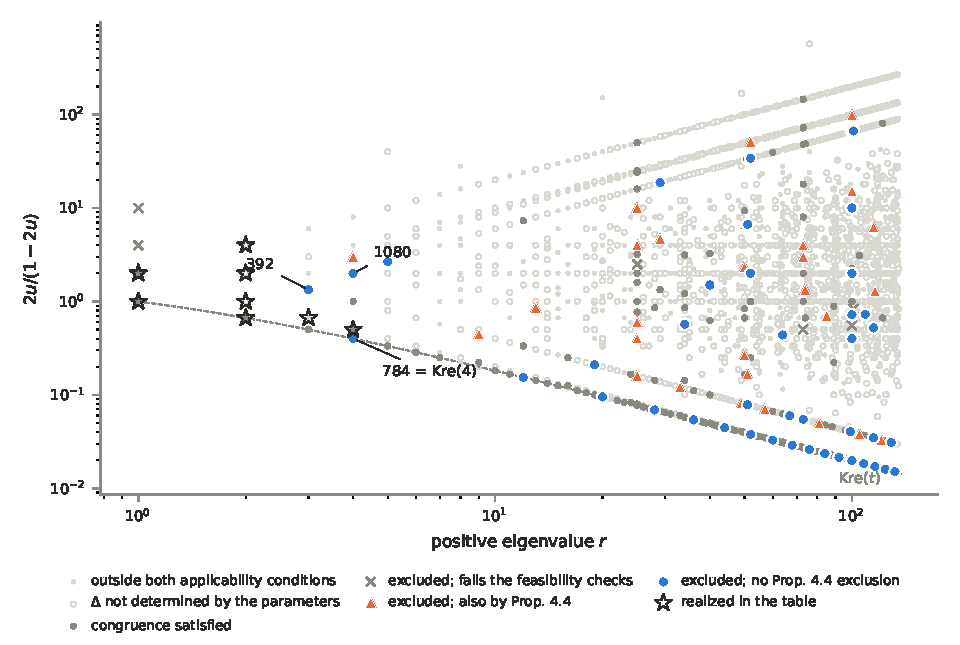
\includegraphics[width=0.92\textwidth]{figures/reach.pdf}
\caption{The $2320$ Smith parameter sets with $r\le135$, plotted against $r$
and $y=2u/(1-2u)=e/(r(r+1))-1$. By Lemma~\ref{lem:param}(iii) a fixed
$u$ gives a horizontal line. $\Kre(t)$ lies on $y=2/(r+1)$ (dashed), series (i)
of Corollary~\ref{cor:series} on $y=4/r$, and $GQ(q,q^2)$ on $y=2/r$. Grey
points record which test was evaluated and its outcome. Stars mark the eight
realized rows of Brouwer's table ($n\le1300$); realized graphs beyond it, such
as $GQ(7,49)$ on $2752$ vertices, are not marked, and none is
excluded.}\label{fig:reach}
\end{figure}

\paragraph{Known graphs.}
No realized parameter set in \cite{Tab} is excluded. Eight realized rows with
integral eigenvalues have $q^s_{ss}=0$ in the orientation listed ($n=16$, $27$,
$100$, $112$, $162$, $275$, $325$, $756$; their complements have
$q^r_{rr}=0$); the pentagon is a ninth. Applying Theorems~\ref{thm:main}
and~\ref{thm:vertex} and Proposition~\ref{prop:second} to all $4538$ rows of
the table and their complements excludes $156$ rows already marked
nonexistent and the six open rows $392$, $784$, $1080$ (and complements), and
nothing else; Theorem~\ref{thm:headline}(d) excludes in addition the two open
rows on $667$ vertices. For $GQ(q,q^2)$ we have $b=q+1$, $br+a=q^2$, $F=q(q+1)^2$ and
$L=q$. For odd $q$, the hypothesis $8\nmid F$ of Theorem~\ref{thm:main}(a) holds
exactly when $q\equiv1\pmod4$; if also every prime divisor of $q$ is
$\equiv1\pmod4$, then $g$ is odd, so $\Delta\equiv\odd(q+1)^{g+1}\equiv1$,
and (a) holds because $(br+a-1)n/F=(q^2-1)n/F\equiv0$. (For $q=9$ the
hypothesis holds but $3\mid L$.) For $q=2$, part (b) applies
and holds. The families of \S\ref{sec:second} were checked by a separate
program: the Pell sequence through twelve qualifying members, and
Theorem~\ref{thm:fixed} and Corollary~\ref{cor:biggs} for all $q<3000$.

\paragraph{Controls.}
The repository also contains controls on known graphs: maximal $2$-integral
lattices for the Higman--Sims graph and $Q^-(5,5)$, which are unimodular and
satisfy Lemma~\ref{lem:charnorm} as predicted, and Theorem~\ref{thm:frame} on
all $769$ rational eigenspaces of $223$ intersection arrays of known
distance-regular graphs.

\section*{Acknowledgments}
We thank Anton Kova\v l for his discriminant-form census and software, which we
used to cross-check the table rows and several parameter sets in
\S\ref{sec:second}. We are especially grateful to him for an independent
verification of this paper: with his own code he rechecked the lattice
results of \S\S\ref{sec:lattices}--\ref{sec:srg}, the four table rows and the
short proofs of \S\ref{sec:intro}, the families of
\S\S\ref{sec:vertex}--\ref{sec:second}, the distance-regular exclusions and the
censuses of \S\ref{sec:checks}, and he tested Theorem~\ref{thm:main} on many
existing graphs. His comments led to several clarifications, among them
Remark~\ref{rem:norton}, the explicit cell data in the proof of
Theorem~\ref{thm:sub}, the list of the projector sums of \S\ref{sec:drg}, and
the precise description of his census in \S\ref{sec:intro}.

%======================================================================
\clearpage
\appendix
\section{Tables}\label{app:tables}

\begin{table}[H]\footnotesize\centering
\caption{The $42$ Smith parameter sets with $n\le10^7$ excluded by
Theorem~\ref{thm:main} (parts (a), (b)) or Theorem~\ref{thm:vertex}. Rows
marked 1.2(a) are members of $\Kre(t)$ whose $L=t$ has a prime divisor
$\equiv3\pmod4$; there $\Delta$ comes from the neighbor basis, as in the proof
of Theorem~\ref{thm:headline}(a). In the
column ``2nd'', P or S records a Proposition~\ref{prop:second} exclusion of the
graph or of a subconstituent, and a dash means no
Proposition~\ref{prop:second} exclusion. ``inf.'' marks the four sets that fail
the feasibility checks. Family labels refer to $\Kre(t)$ and to
Corollary~\ref{cor:series}.}\label{tab:scan}
\setlength{\tabcolsep}{4pt}
\begin{tabular}{rrrrrrrlcl}\toprule
$n$&$k$&$\lambda$&$\mu$&$r$&$u$&$g$&test&2nd&family\\\midrule
50&21&4&12&1&2/5&7&1.1(a)&P&(i) $t{=}2$, inf.\\
121&56&15&35&1&5/11&8&1.1(b)&--&inf.\\
392&115&18&40&3&2/7&46&1.1(a)&--&(i) $t{=}4$\\
784&116&0&20&4&1/7&116&1.1(a)&--&$\Kre(4)$\\
1080&364&88&140&4&1/3&78&1.1(a)&--&(ii) $t{=}4$\\
1408&532&156&228&4&3/8&77&6.1&S&\\
2420&885&260&360&5&4/11&118&1.1(a)&--&\\
8450&1309&108&220&9&2/13&595&1.1(a)&P&(i) $t{=}10$\\
24167&5590&1053&1365&13&3/13&946&1.1(b)&P&\\
32400&2172&0&156&12&1/15&2172&1.2(a)&--&$\Kre(12)$\\
105800&9219&418&840&19&2/23&4390&1.1(a)&--&(i) $t{=}20$\\
167680&31465&5100&6090&25&3/16&4061&6.1&S&\\
181545&25960&2975&3835&25&1/7&5016&1.1(b)&S&\\
211600&9220&0&420&20&1/23&9220&1.1(a)&--&$\Kre(20)$\\
248430&88750&30275&32500&25&5/14&2769&1.1(a)&--&inf.\\
284258&19629&700&1404&25&2/29&9451&1.1(a)&P&(i) $t{=}26$\\
341250&136525&52700&55900&25&2/5&2667&1.1(a)&P&\\
421685&76704&12478&14280&34&2/11&7708&1.1(b)&--&\\
595051&245050&98049&102921&29&7/17&3550&1.1(b)&P&\\
731445&332500&147275&154375&25&5/11&2604&1.1(b)&S&\\
753424&24332&0&812&28&1/31&24332&1.2(a)&--&$\Kre(28)$\\
779000&233740&67320&71340&40&3/10&7657&6.1&--&\\
791282&42805&1188&2380&33&2/37&20791&1.1(a)&P&(i) $t{=}34$\\
1691285&178080&15950&19080&50&2/19&26236&1.1(b)&S&\\
1870000&654550&223650&232050&50&7/20&11077&6.1&S&\\
1934712&644956&209560&217724&52&1/3&12246&1.1(a)&--&(ii) $t{=}52$\\
1971216&50580&0&1332&36&1/39&50580&1.2(a)&--&$\Kre(36)$\\
2018980&958189&445788&462840&29&28/59&3478&1.1(a)&--&\\
2342396&167365&9180&12172&51&1/14&38665&1.1(a), 6.1&S&\\
2941240&447644&63168&69020&64&7/46&31553&6.1&--&\\
3511250&132549&2548&5100&49&2/53&64975&1.1(a)&P&(i) $t{=}50$\\
4001885&1740000&745550&765000&50&10/23&10324&1.1(b)&S&\\
4089800&148771&2754&5512&51&2/55&72982&1.1(a)&--&(i) $t{=}52$\\
4229766&705034&110887&118844&73&1/6&38193&1.1(a)&--&inf.\\
4244696&1845571&791010&811240&51&10/23&10738&1.1(a)&--&\\
4276624&91036&0&1980&44&1/47&91036&1.2(a)&--&$\Kre(44)$\\
4686605&1339104&373478&386280&74&2/7&26884&1.1(b)&S&\\
6258722&205261&3420&6844&57&2/61&100891&1.1(a)&P&(i) $t{=}58$\\
6432103&1321750&261885&274125&85&15/73&44162&1.1(b)&P&\\
6741696&2528209&934692&956154&73&3/8&22893&6.1&S&\\
8179600&148772&0&2756&52&1/55&148772&1.1(a)&--&$\Kre(52)$\\
8238050&3295293&1302028&1328892&73&2/5&22387&1.1(a)&P&\\
\bottomrule
\end{tabular}
\end{table}

\begin{table}[H]\scriptsize\centering
\caption{Intersection arrays in the BCN tables \cite{DRGtab} with an eigenspace
failing Theorem~\ref{thm:frame}. Where two eigenvalues are listed, $(\gamma_i)$ and
``cubic'' ($\sum k_i\gamma_i^3=0$) refer to the first. The last column names a
strongly regular graph that the array would produce (by a fusion of distance
classes, folding, or the complement of a halved graph), and where that graph
is excluded; Proposition~\ref{prop:second} does not apply to the graph at
$616$.}\label{tab:drg}
\setlength{\tabcolsep}{1.7pt}
\begin{tabular}{rlrrrlcl}\toprule
$n$&array&$\theta$&$m$&$F$&$(\gamma_i)$&cubic&derived graph\\\midrule
50&$\{14,10,3;1,5,12\}$&$-6,\ 4$&7, 14&50&$(7,-3,2,-3)$&yes&$(50,21,4,12)$, abs.\ bound\\
350&$\{30,22,9;1,3,20\}$&$0,\ -5$&154, 132&50, 175&$(22,0,-1,2)$&no&Ex.~\ref{ex:shilla}\\
392&$\{69,56,10;1,14,60\}$&$-15$&46&196&$(23,-5,2,-5)$&yes&$(392,115,18,40)$\\
525&$\{40,33,3;1,3,30\}$&$-5,\ 5$&308, 132&150, 350&$(88,-11,1,-2)$&no&\\
616&$\{90,60,12;1,12,72\}$&$2$&252&550&$(225,5,-6,27)$&no&$(616,165,44,44)$: open\\
750&$\{112,77,16;1,16,88\}$&$-8$&308&375&$(154,-11,4,-11)$&no&$(750,210,55,60)$ \cite{Koval}\\
1014&$\{78,77,65,8;1,13,70,78\}$&$-13,\ 13$&198&338&$(66,-11,1,2,-12)$&no&$(507,44,1,4)$ \cite{Koval}\\
1960&$\{115,96,32,1;1,8,96,115\}$&$-25$&46&980&$(23,-5,2,-5,23)$&yes&$(392,115,18,40)$\\
3920&$\{116,115,16,1;1,4,115,116\}$&$-24$&116&980&$(29,-6,1,-6,29)$&yes&$\Kre(4)$\\
4732&$\{165,160,6,1;1,6,160,165\}$&$15,\ -11$&1001, 1365&52&$(11,1,0,-1,-11)$&yes&$(4732,166,0,6)$, Thm.~\ref{thm:fixed}\\
5046&$\{261,260,232,21;1,29,240,261\}$&$-29,\ 29$&702&1682&$(234,-26,2,3,-27)$&no&$(2523,182,1,14)$, Prop.~\ref{prop:second}\\
8450&$\{594,550,45,1;1,45,550,594\}$&4 values&&&&&\cite{CW}\\
11774&$\{406,405,377,16;1,29,390,406\}$&$-29,\ 29$&2646&1682&$(378,-27,1,2,-28)$&no&$(5887,216,5,8)$, Prop.~\ref{prop:second}\\
\bottomrule
\end{tabular}
\end{table}

\FloatBarrier

\begin{thebibliography}{99}
\bibitem{Akiyama} K.~Akiyama, Nonexistence of a strongly regular graph with
parameters $(266,45,0,9)$: a certificate-free Lean proof, arXiv:2609.08319
(2026).
\bibitem{AM} J.~Azarija and T.~Marc, There is no $(75,32,10,16)$ strongly
regular graph, \emph{Linear Algebra Appl.} 557 (2018) 62--83.
\bibitem{BMV} E.~Bannai, A.~Munemasa and B.~Venkov, The nonexistence of
certain tight spherical designs, \emph{Algebra i Analiz} 16(4) (2004) 1--23;
English translation: \emph{St.\ Petersburg Math.\ J.} 16 (2005) 609--625.
\bibitem{Biggs} N.~Biggs, Strongly regular graphs with no triangles,
arXiv:0911.2160 (2009).
\bibitem{Biggs2} N.~Biggs, Families of parameters for SRNT graphs,
arXiv:0911.2455 (2009).
\bibitem{Biggs3} N.~Biggs, The second subconstituent of some strongly regular
graphs, arXiv:1003.0175 (2010).
\bibitem{BR} A.~V. Bondarenko and D.~V. Radchenko, On a family of strongly
regular graphs with $\lambda=1$, \emph{J.\ Combin.\ Theory Ser.\ B} 103
(2013) 521--531.
\bibitem{BPR} A.~V. Bondarenko, A.~Prymak and D.~Radchenko, Non-existence of
$(76,30,8,14)$ strongly regular graph, \emph{Linear Algebra Appl.} 527 (2017)
53--72.
\bibitem{Br77} A.~E. Brouwer, The uniqueness of the strongly regular graph on
$77$ points, \emph{J.\ Graph Theory} 7 (1983) 455--461.
\bibitem{BCN} A.~E. Brouwer, A.~M. Cohen and A.~Neumaier,
\emph{Distance-Regular Graphs}, Springer, 1989.
\bibitem{DRGtab} A.~E. Brouwer, Parameters of distance-regular graphs
(machine-readable BCN tables), \url{https://www.win.tue.nl/~aeb/drg/},
downloaded 22 November 2026.
\bibitem{Tab} A.~E. Brouwer, Parameters of strongly regular graphs,
\url{https://aeb.win.tue.nl/graphs/srg/}, accessed 18 November 2026.
\bibitem{BvM} A.~E. Brouwer and H.~Van Maldeghem, \emph{Strongly Regular
Graphs}, Cambridge University Press, 2022.
\bibitem{Cameron} P.~J. Cameron, Extending symmetric designs, \emph{J.\
Combin.\ Theory Ser.\ A} 14 (1973) 215--220.
\bibitem{CGS78} P.~J. Cameron, J.-M. Goethals and J.~J. Seidel, The Krein
condition, spherical designs, Norton algebras and permutation groups,
\emph{Indag.\ Math.} 40 (1978) 196--206.
\bibitem{CGS} P.~J. Cameron, J.-M. Goethals and J.~J. Seidel, Strongly regular
graphs having strongly regular subconstituents, \emph{J.\ Algebra} 55 (1978)
257--280.
\bibitem{Cassels} J.~W.~S. Cassels, \emph{Rational Quadratic Forms}, Academic
Press, 1978.
\bibitem{CW} P.~Cesarz and J.~Williford, Four class association scheme double
covers of strongly regular graphs, arXiv:2610.05420 (2026).
\bibitem{CMN} M.~Chen, A.~A. Makhnev and M.~S. Nirova, On graphs in which the
neighborhoods of vertices are edge-regular graphs without $3$-claws,
\emph{Trudy Inst.\ Mat.\ Mekh.\ UrO RAN} 29(4) (2023) 279--282; English
translation: \emph{Proc.\ Steklov Inst.\ Math.} 323 (Suppl.~1) (2023)
S53--S55.
\bibitem{CS} J.~H. Conway and N.~J.~A. Sloane, \emph{Sphere Packings, Lattices
and Groups}, 3rd ed., Springer, 1999.
\bibitem{CJ} K.~Coolsaet and A.~Juri\v si\'c, Using equality in the Krein
conditions to prove nonexistence of certain distance-regular graphs, \emph{J.\
Combin.\ Theory Ser.\ A} 115(6) (2008) 1086--1095.
\bibitem{DGS} P.~Delsarte, J.-M. Goethals and J.~J. Seidel, Spherical codes and
designs, \emph{Geom.\ Dedicata} 6 (1977) 363--388.
\bibitem{EM} K.~S. Efimov and A.~A. Makhnev, Automorphisms of a
distance-regular graph with intersection array $\{30,22,9;1,3,20\}$,
\emph{Trudy Inst.\ Mat.\ Mekh.\ UrO RAN} 26(3) (2020) 23--31; English
translation: \emph{Proc.\ Steklov Inst.\ Math.} (2021),
doi:10.1134/S0081543821060080.
\bibitem{GM} A.~L. Gavrilyuk and A.~A. Makhnev, On Krein graphs without
triangles, \emph{Dokl.\ Math.} 72 (2005) 591--594.
\bibitem{GVW} A.~L. Gavrilyuk, J.~Vidali and J.~S. Williford, On few-class
$Q$-polynomial association schemes: feasible parameters and nonexistence
results, \emph{Ars Math.\ Contemp.} 20(1) (2021) 103--127.
\bibitem{KO} P.~Kaski and P.~R.~J. \"Osterg\aa rd, There are exactly five
biplanes with $k=11$, \emph{J.\ Combin.\ Des.} 16 (2008) 117--127.
\bibitem{Koval} A.~Kova\v l, The Bannai--Munemasa--Venkov lattice method for
strongly regular graphs: a uniform discriminant-form condition and new
nonexistence results, preprint and data, 2026,
\url{https://doi.org/10.5281/zenodo.23281359}.
\bibitem{LM} J.~Lansdown and W.~J. Martin, Rational Delsarte designs and
Galois fusions of association schemes, \emph{Canad.\ Math.\ Bull.} (2025);
arXiv:2406.06991.
\bibitem{Makhnev} A.~A. Makhnev, The graph $\Kre(4)$ does not exist,
\emph{Dokl.\ Math.} 96 (2017) 348--350.
\bibitem{MN} A.~A. Makhnev and V.~V. Nosov, Automorphisms of strongly regular
Krein graphs without triangles, \emph{Algebra Logic} 44 (2005) 185--196.
\bibitem{MP} A.~A. Makhnev and D.~V. Paduchikh, Strongly regular graphs with
strongly regular local subgraphs having second eigenvalue $5$, talk at the
conference Groups and Graphs, Algorithms and Automata, Yekaterinburg, 2015.
\bibitem{MH} J.~Milnor and D.~Husemoller, \emph{Symmetric Bilinear Forms},
Springer, 1973.
\bibitem{NV} G.~Nebe and B.~Venkov, On tight spherical designs,
\emph{Algebra i Analiz} 24(3) (2012) 163--171; English translation:
\emph{St.\ Petersburg Math.\ J.} 24 (2013) 485--491.
\bibitem{OMeara} O.~T. O'Meara, \emph{Introduction to Quadratic Forms},
Springer, 1963.
\bibitem{Scott} L.~L. Scott, A condition on Higman's parameters, \emph{Notices
Amer.\ Math.\ Soc.} 20 (1973) A-97.
\bibitem{Smith} M.~S. Smith, On rank $3$ permutation groups, \emph{J.\
Algebra} 33 (1975) 22--42.
\bibitem{vdB} F.~van der Blij, An invariant of quadratic forms mod $8$,
\emph{Indag.\ Math.} 21 (1959) 291--293.
\bibitem{Venkov} B.~Venkov, R\'eseaux et designs sph\'eriques, in
\emph{R\'eseaux euclidiens, designs sph\'eriques et formes modulaires},
Monogr.\ Enseign.\ Math.\ 37, Geneva, 2001, 10--86.
\end{thebibliography}
\end{document}
